\chapter{HASIL DAN PEMBAHASAN}
\label{chap:chap4_eval}
\vspace{1ex}


\section*{}
Inti dari BAB \ref{chap:chap4_eval} pada penelitian ini adalah pengujian dengan berbagai parameter \textit{stats} yang dihasilkan untuk pemain dan musuh. Jika pada BAB \ref{chap:chap3_metodologi} dalam proses analisan desain permainan RPG, permainan RPG digolongkan berdasarkan pertarungan menjadi \textit{real-time} dan \textit{turn-based}.
\vspace{1ex}

Kemudian jika melihat jumlah karakter yang dimainkan oleh pemain maka permainan RPG dapat digolongkan menjadi \textit{single-character} dan \textit{multi-character}. Hal ini diperlukan dalam pengujian pembuatan \textit{stats} yang dihasilkan, permainan RPG yang termasuk \textit{single-character} adalah WRPG, ARPG, SRPG dan MMORPG, sedangkan yang termasuk \textit{multi-character} adalah TRPG dan JRPG. Sedangkan untuk karakter musuh dianggap sama, hanya saja dalam beberapa permainan bergenre RPG pemain dan musuh tidak menggunakan sistem elemen sebagai kelemahan. Biasanya pada permainan RPG dengan genre ARPG, SRPG dan sebagian WRPG, sedangkan untuk TRPG dan JRPG hampir sebagian besar memakai sistem elemen sebagai kelemahan dalam sistem pertarungan.
\vspace{1ex}

\section{Pembuatan Stats Single-Character untuk Pemain}
\label{sec:sec4_eval_single-character_player}
\vspace{1ex}

Pada bagian ini setiap langkah yang akan diuji sudah dijelaskan pada Sub-bab \ref{sec:sec3_player_stats}, dimana pada bagian ini membahas tentang pembuatan \textit{stats} pemain untuk permaian bergenre RPG. Melalui berbagai proses seperti yang dijelaskan pada Sub-bab \ref{sec:sec3_player_stats}, maka pada beberapa Sub-bab dibawah ini adalah langkah-langkah dalam proses pengujiannya. Maksud dari \textit{single-character} disini adalah pemain hanya menjalankan satu buah karakter saja selama permainan, contoh dari RPG jenis ini biasanya ada pada WRPG, SRPG, ARPG, dan MMORPG.
\vspace{1ex}

\subsection{Distibusi Level, HP, dan MP Pemain}
\label{sec:sub_sec4_eval_dist_hp_mp_level_single-character}
\vspace{1ex}

Seperti yang sudah dijelaskan pada Sub-bab \ref{sec:sub_sec3_player_level_hp_mp}, dimana pada bagian ini membahas tentang pembuatan level, HP dan MP pemain untuk permaian dengan genre RPG. Berikut adalah hasil dari prosess pembuatan Level, HP, dan MP yang diperoleh dari perhitungan pada persamaan \ref{eq:hp_player} dan \ref{eq:mp_player} dengan data masukan pada Tabel \ref{tb:player_input_variable} yang kemudian menghasilkan data seperti yang ditunjukkan pada Tabel \ref{tb:player_hp_mp}.

\begin{longtable}{|l|l|l|}
	\caption{Hasil Perhitungan HP dan MP}
	\vspace{1ex}
	\label{tb:player_hp_mp}\\
	\hline
	\rowcolor[HTML]{C0C0C0} 
	\textbf{Levels} & \textbf{HP} & \textbf{MP} \\ \hline
	1 & 159 & 89 \\ \hline
	2 & 163 & 93 \\ \hline
	3 & 167 & 97 \\ \hline
	4 & 171 & 101 \\ \hline
	5 & 175 & 105 \\ \hline
	6 & 179 & 109 \\ \hline
	7 & 183 & 113 \\ \hline
	... & ... & ... \\ \hline
	\textbf{100} & \textbf{555} & \textbf{485} \\ \hline
\end{longtable}
\vspace{1ex}

Hasil perhitungan tersebut terlihat membentuk pola linier, yang mana nilai HP dan MP terus naik secara konstan ke atas sesuai dengan kenaikan levelnya seperti yang direpresentasikan pada Gambar \ref{fig:hp_player} dan Gambar \ref{fig:mp_player}. Jika melihat Gambar \ref{fig:hp_player} dengan jumlah HP dari pemain yang terus naik mengikuti pola yang dihasilkan pada Tabel \ref{tb:player_hp_mp}, yang mana nilai tersebut diperoleh dari inisiasi variabel pada Tabel \ref{tb:player_input_variable} yaitu \textit{Max Level}, \textit{Start} HP dan \textit{Next} HP. Variabel-variabel tersebut dihitung dengan menggunakan persamaan \ref{eq:hp_player} agar membentuk pola kenaikan HP setiap levelnya seperti yang ditunjukan pada Gambar \ref{fig:hp_player}. Sama seperti pada Gambar \ref{fig:hp_player}, pada Gambar \ref{fig:mp_player} dengan jumlah MP dari pemain yang terus naik mengikuti pola yang dihasilkan pada Tabel \ref{tb:player_hp_mp}, yang mana nilai tersebut diperoleh dari inisiasi variabel pada Tabel \ref{tb:player_input_variable} yaitu \textit{Max Level}, \textit{Start} MP dan \textit{Next} MP. Kemudian variabel-variabel tersebut dihitung dengan menggunakan persamaan \ref{eq:mp_player} agar membentuk pola kenaikan MP setiap levelnya seperti yang ditunjukan pada Gambar \ref{fig:mp_player}. 
\vspace{1ex}

\begin{figure} [!h] \centering
	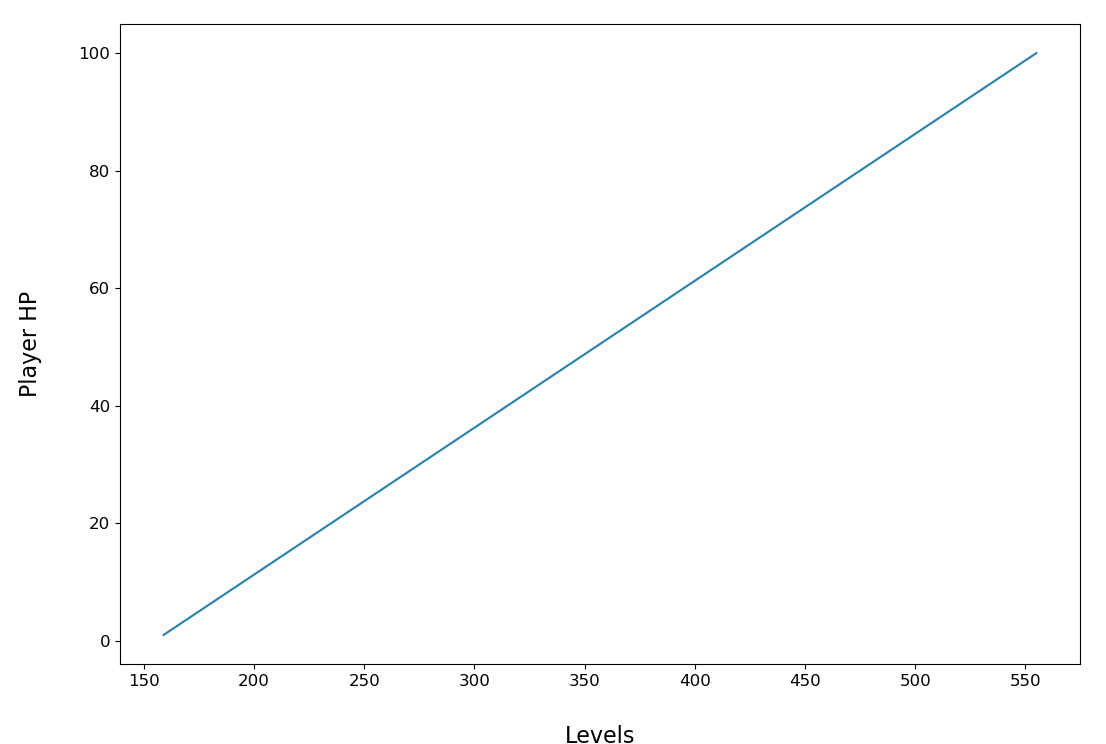
\includegraphics[scale=0.44]{img/PlayerHpDistrib.png}
	\caption{Kenaikan HP setiap levelnya.}
	\label{fig:hp_player}
\end{figure}

\begin{figure} [!h] \centering
	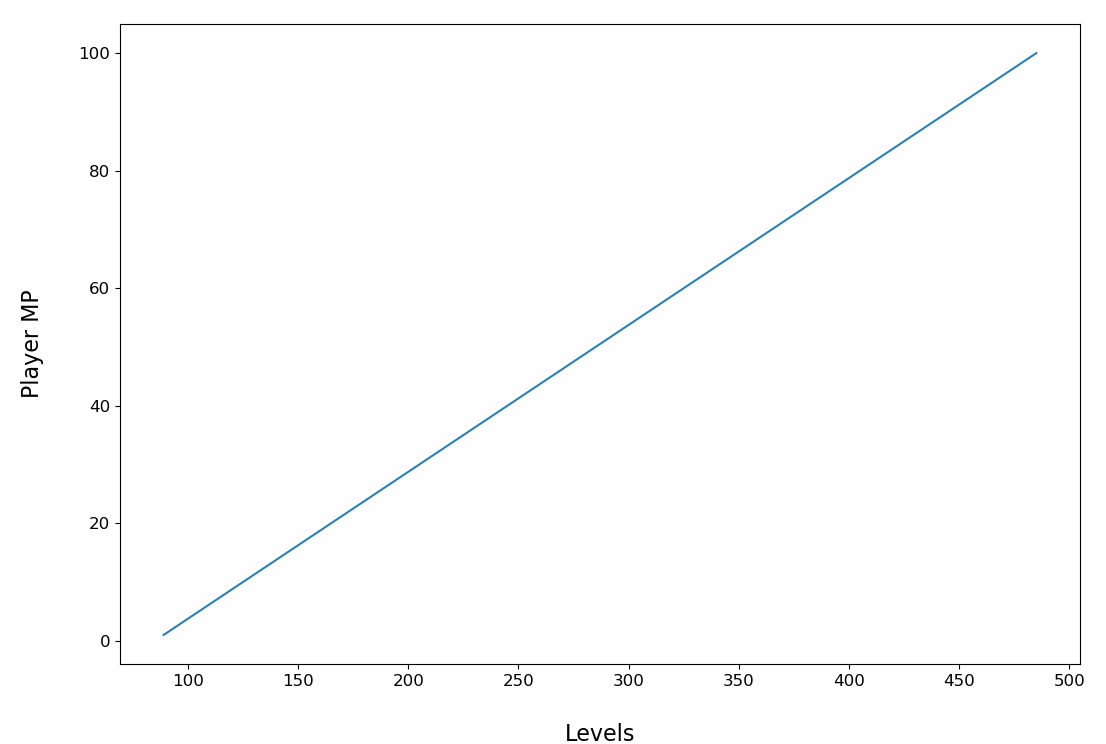
\includegraphics[scale=0.44]{img/PlayerMpDistrib.png}
	\caption{Kenaikan MP setiap levelnya.}
	\label{fig:mp_player}
\end{figure}

Pada setiap proses pengujian dalam Sub-bab ini, yang dihasilkan pada Tabel \ref{tb:player_hp_mp} menyajikan sebagian data saja. Hasil selengkapnya dapat dilihat pada Tabel \ref{tb:player_hp_mp_all} dalam \nameref{chap:chap6_attachment} yang kemudian keseluruhan hasil tersebut divisualisasikan pada Gambar \ref{fig:hp_player}.
\vspace{1ex}

\subsection{Distibusi Elemen dan Kelemahan Pemain}
\label{sec:sub_sec4_eval_dist_element_single-character}
\vspace{1ex}

Pada bagian ini hanya akan mengulas tentang distribusi elemen dan kelemahan pemain pada Sub-Bab \ref{sec:sub_sec3_list_element_player}, yang sejatinya didefinisikan secara manual pada program yang dibuat dan dijelaskan pada Sub-Bab \ref{sec:sec3_player_stats}. Di mana elemen pada permainan RPG bersifat opsional, tidak dibatasi apakah permainan RPG tersebut tergolong ke dalam \textit{turn-base} atau \textit{real-time}, tergolong \textit{singe-character} atau \textit{multi-character}. Hal tersebut murni bergantung pada pengembang dan desainer permainan. Maka dari itu melalui program yang dibuat pada Sub-Bab \ref{sec:sec3_player_stats} hal ini diwujudkan dalam bentuk opsi yang dapat digunakan atau ditinggalkan, sesuai kebutuhan pengembang atau desainer permainan. Bila opsi distribusi elemen digunakan maka hasilnya akan tampak seperti pada Tabel \ref{tb:player_element}, dengan asumsi tidak adanya perubahan elemen dari karakter pemain dalam permainan.
\vspace{-1ex}

\begin{longtable}{|l|l|l|l|l|l|}
	\caption{Distribusi elemen pada karakter pemain}
	\vspace{1ex}
	\label{tb:player_element}\\
	\hline
	\rowcolor[HTML]{C0C0C0} 
	\multicolumn{1}{|c|}{\cellcolor[HTML]{C0C0C0}\textbf{Levels}} & \multicolumn{1}{c|}{\cellcolor[HTML]{C0C0C0}\textbf{Water}} & \multicolumn{1}{c|}{\cellcolor[HTML]{C0C0C0}\textbf{Wind}} & \multicolumn{1}{c|}{\cellcolor[HTML]{C0C0C0}\textbf{Earth}} & \multicolumn{1}{c|}{\cellcolor[HTML]{C0C0C0}\textbf{Fire}} \\ \hline
	1 & 2 & 0 & 0 & 1 \\ \hline
	2 & 2 & 0 & 0 & 1 \\ \hline
	3 & 2 & 0 & 0 & 1 \\ \hline
	4 & 2 & 0 & 0 & 1 \\ \hline
	5 & 2 & 0 & 0 & 1 \\ \hline
	6 & 2 & 0 & 0 & 1 \\ \hline
	7 & 2 & 0 & 0 & 1 \\ \hline
	... & ... & ... & ... & ... \\ \hline
	\textbf{100} & \textbf{2} & \textbf{0} & \textbf{0} & \textbf{1} \\ \hline
\end{longtable}

Pada setiap proses pengujian dalam Sub-bab ini, yang dihasilkan pada Tabel \ref{tb:player_element} menyajikan sebagian data saja. Hasil selengkapnya dapat dilihat pada Tabel \ref{tb:player_all_stats_1} sampai dengan Tabel \ref{tb:player_all_stats_4} dalam \nameref{chap:chap6_attachment}. Hal seperti penggunaan elemen pada pemain seperti pembahasan pada Sub-bab ini an sebelumnya, biasanya dijumpai pada permain RPG dengan Sub-genre JRPG, TRPG, WRPG dan MMORPG. Namun itu juga tidak semua permainan RPG dengan genre tersebut menggunakannya, hanya yang sering dijumpai saja.
\vspace{1ex}

\subsection{Pengujian Distibusi Stats Pemain}
\label{sec:sub_sec4_eval_single-character_stats}
\vspace{1ex}

Pada bagian ini setiap langkah yang akan diuji sudah dijelaskan pada Sub-bab \ref{sec:sub_sec3_stat_pemain}, dimana pada bagian ini membahas tentang pembuatan \textit{stats} pemain untuk permaian RPG. Melalui berbagai proses seperti yang dijelaskan pada Sub-bab \ref{sec:sub_sec3_stat_pemain}, melalui data masukan pada Tabel \ref{tb:player_input_variable} kemudian persamaan \ref{eq:KNN_bayes_player_stats} dan beberapa persamaan lain yang disebutkan pada Sub-bab \ref{sec:sub_sec3_stat_pemain} dihasilkan data seperti yang ditunjukan pada Tabel \ref{tb:player_battle_stats}.
\vspace{-1ex}

\begin{longtable}{|l|l|l|l|l|l|}
	\caption{Distribusi stats pada karakter pemain}
	\vspace{1ex}
	\label{tb:player_battle_stats}\\
	\hline
	\rowcolor[HTML]{C0C0C0} 
	\textbf{Levels} & \textbf{Strength} & \textbf{Magic} & \textbf{Endurance} & \textbf{Speed} & \textbf{Luck} \\ \hline
	1 & 1 & 2 & 0 & 0 & 1 \\ \hline
	2 & 0 & 2 & 0 & 2 & 0 \\ \hline
	3 & 1 & 0 & 0 & 0 & 0 \\ \hline
	4 & 1 & 1 & 0 & 0 & 0 \\ \hline
	5 & 1 & 1 & 0 & 0 & 0 \\ \hline
	6 & 1 & 1 & 0 & 2 & 1 \\ \hline
	7 & 0 & 0 & 0 & 0 & 1 \\ \hline
	... & ... & ... & ... & ... & ... \\ \hline
	\textbf{100} & \textbf{74} & \textbf{38} & \textbf{63} & \textbf{65} & \textbf{60} \\ \hline
\end{longtable}
\vspace{1ex}

Pada Tabel \ref{tb:player_battle_stats} adalah data \textit{stats} dari pemain yang dihasilakn melalui penambahan nilai pada \textit{stats} secara acak pada setiap \textit{stats}. Seperti yang dijelaskan pada persaamaan \ref{eq:nbayes_class}, \ref{eq:KNN_distance_stats}, dan persamaan \ref{eq:KNN_bayes_player_stats} saat nilai \textit{stats} di tambahkan secara acak dari 1 sampai dengan 2 pada level yang berjarak antara 1 sampai dengan 100. Selanjutnya representasi dari hasil penambahan \textit{stats} tersebut yang ditunjukan melalui Gambar \ref{fig:stats_player} yang mana nilai dari setiap \textit{stats} terus naik sesuai dengan level pemain yang juga terus naik. 
\vspace{1ex}

\begin{figure} [!h] \centering
	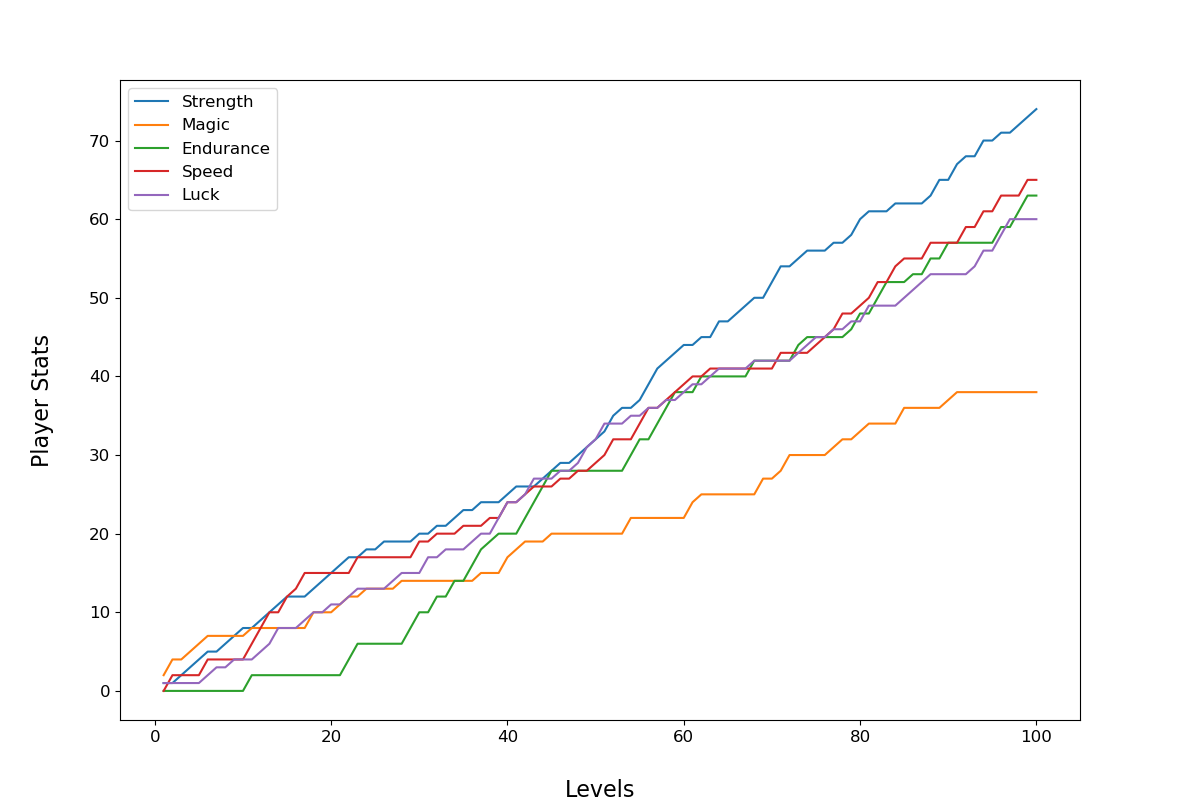
\includegraphics[scale=0.50]{img/PlayerStatsDistrib.png}
	\caption{Kenaikan stats pemain setiap levelnya.}
	\label{fig:stats_player}
\end{figure}

Pada setiap proses pengujian dalam Sub-bab ini, yang dihasilkan pada Tabel \ref{tb:player_battle_stats} menyajikan sebagian data saja. Hasil selengkapnya dapat dilihat pada Tabel \ref{tb:player_all_stats_1} sampai dengan Tabel \ref{tb:player_all_stats_4} dalam \nameref{chap:chap6_attachment} yang kemudian keseluruhan hasil tersebut divisualisasikan pada Gambar \ref{fig:stats_player}.
\vspace{1ex}

\section{Pembuatan Stats Multi-Character untuk Pemain}
\label{sec:sec4_eval_multi-character_player}
\vspace{1ex}

Pada bagian ini setiap langkah yang akan diuji sudah dijelaskan pada Sub-bab \ref{sec:sec3_player_stats}, dimana pada bagian ini membahas tentang pembuatan \textit{stats} pemain untuk permaian dengan genre RPG. Melalui berbagai proses seperti yang dijelaskan pada Sub-bab \ref{sec:sec3_player_stats}, maka pada beberapa Sub-bab dibawah ini adalah langkah-langkah dalam proses pengujiannya. Maksud dari Multi-Character disini adalah pemain dapat menjalankan beberapa karakter sekaligus, menjalankan dengan mode \textit{turn-based} atau \textit{switch} antar karakter seperti yang dijelaskan pada Sub-Bab \ref{sec:sub_sec2_jrpg}. Maka dari itu dibuatlah Tabel masukan baru pada Tabel \ref{tb:player_input_variable_eval_1} dan \ref{tb:player_input_variable_eval_2} yang mirip seperti Tabel \ref{tb:player_input_variable}. Hal ini bertujuan membandingkan perbedaan \textit{stats} yang dihasilkan pada tiga karakter pemain.
\vspace{-1ex}

\begin{longtable}{|l|l|}
	\caption{Data masukan untuk pembuatan \textit{stats} karakter pertama.}
	\vspace{1ex}
	\label{tb:player_input_variable_eval_1}\\
	\hline
	\rowcolor[HTML]{9B9B9B}
	\multicolumn{1}{|c|}{\cellcolor[HTML]{9B9B9B}\textbf{Variabel}} & \multicolumn{1}{c|}{\cellcolor[HTML]{9B9B9B}\textbf{Input}} \\ \hline
	\textit{Start} Level & 1 \\ \hline
	\textit{Max} Level & 100 \\ \hline
	\textit{Start} HP & 224 \\ \hline
	\textit{Next} HP & 228 \\ \hline
	\textit{Start} MP & 100 \\ \hline
	\textit{Next} MP & 102 \\ \hline
	\textit{List Element} & {[} `Phys', `Water', `Wind', `Earth', `Fire' {]} \\ \hline
	\textit{List Weaknesess} & {[} 0, 0, 2, 1, 0 {]} \\ \hline
	\textit{List Stats Name} & {[} `Strength', `Magic', `Endurance', `Speed', `Luck' {]} \\ \hline
	\textit{Max Stats Value} & {[} 88, 32, 81, 43, 56 {]} \\ \hline
	\textit{Stats to Assign} & {[} 2, 1 {]} \\ \hline
\end{longtable}
\vspace{-1ex}

\begin{longtable}{|l|l|}
	\caption{Data masukan untuk pembuatan \textit{stats} karakter kedua.}
	\vspace{1ex}
	\label{tb:player_input_variable_eval_2}\\
	\hline
	\rowcolor[HTML]{9B9B9B} 
	\multicolumn{1}{|c|}{\cellcolor[HTML]{9B9B9B}\textbf{Variabel}} & \multicolumn{1}{c|}{\cellcolor[HTML]{9B9B9B}\textbf{Input}} \\ \hline
	\textit{Start} Level & 1 \\ \hline
	\textit{Max} Level & 100 \\ \hline
	\textit{Start} HP & 223 \\ \hline
	\textit{Next} HP & 226 \\ \hline
	\textit{Start} MP & 154 \\ \hline
	\textit{Next} MP & 158 \\ \hline
	\textit{List Element} & {[} `Phys', `Water', `Wind', `Earth', `Fire' {]} \\ \hline
	\textit{List Weaknesess} & {[} 0, 1, 0, 0, 2 {]} \\ \hline
	\textit{List Stats Name} & {[} `Strength', `Magic', `Endurance', `Speed', `Luck' {]} \\ \hline
	\textit{Max Stats Value} & {[} 60, 68, 57, 58, 57 {]} \\ \hline
	\textit{Stats to Assign} & {[} 2, 1 {]} \\ \hline
\end{longtable}
\vspace{1ex}

Kemudian dari Tabel \ref{tb:player_input_variable_eval_1} dan \ref{tb:player_input_variable_eval_2} dihasilkan dua \textit{stats} yang berbeda untuk dua karakter dari pemain. Pada mulanya pemilihan \textit{stats} pemain yang dinyatakan pada ke dua Table tersebut bukanlah tidak beralasan, bila melihat pada Tabel yang sebelumnya dipakai untuk pengujian \textit{single-character} pada Sub-bab \ref{sec:sec4_eval_single-character_player} dan penjabaran metodologi pembuatan \textit{stats} karakter pemain pada Sub-bab \ref{sec:sec3_player_stats} tentu saja masih berkaitan. Ketiga \textit{stats} tersebut membentuk sebuah \textit{party member} dalam permainan JRPG atau bahkan TRPG, hal ini sengaja dibuat dikarenakan hanya genre permainan RPG tersebut yang memungkinkan pemain menggunakan lebih dari satu karakter. Penjelasaan dan penggunaan dari ke empat \textit{stats} tersebut akan diperjelas pada beberapa Sub-bab berikut ini.
\vspace{1ex}

\subsection{Distibusi Level, HP, dan MP Pemain}
\label{sec:sub_sec4_eval_dist_hp_mp_level_multi-character}
\vspace{1ex}

Seperti yang sudah dijelaskan pada Sub-bab \ref{sec:sub_sec3_player_level_hp_mp}, dimana pada bagian ini membahas tentang pembuatan level, HP dan MP pemain untuk permaian dengan genre RPG. Sama seperti pembahasan pada Sub-bab \ref{sec:sub_sec4_eval_dist_hp_mp_level_single-character}, hanya saja pada bagian ini, karakter pemain berjumlah lebih banyak dari pembahasan sebelumnya. Berikut adalah hasil dari prosess pembuatan Level, HP, dan MP yang diperoleh dari perhitungan pada persamaan \ref{eq:hp_player} dan \ref{eq:mp_player} dengan data masukan pada Tabel \ref{tb:player_input_variable_eval_1} dan \ref{tb:player_input_variable_eval_2} yang kemudian menghasilkan data seperti yang ditunjukkan pada Tabel \ref{tb:player_hp_mp_1} dan \ref{tb:player_hp_mp_2}.
\vspace{-1ex}

\begin{longtable}{|l|l|l|}
	\caption{Hasil Perhitungan HP dan MP karakter pertama}
	\vspace{1ex}
	\label{tb:player_hp_mp_1}\\
	\hline
	\rowcolor[HTML]{C0C0C0} 
	\textbf{Levels} & \textbf{HP} & \textbf{MP} \\ \hline
	1 & 224 & 100 \\ \hline
	2 & 228 & 102 \\ \hline
	3 & 232 & 104 \\ \hline
	4 & 236 & 106 \\ \hline
	5 & 240 & 108 \\ \hline
	6 & 244 & 110 \\ \hline
	7 & 248 & 112 \\ \hline
	... & ... & ... \\ \hline
	\textbf{100} & \textbf{620} & \textbf{298} \\ \hline
\end{longtable}
\vspace{-1ex}

\begin{longtable}{|l|l|l|}
	\caption{Hasil Perhitungan HP dan MP karakter kedua}
	\vspace{1ex}
	\label{tb:player_hp_mp_2}\\
	\hline
	\rowcolor[HTML]{C0C0C0} 
	\textbf{Levels} & \textbf{HP} & \textbf{MP} \\ \hline
	1 & 223 & 154 \\ \hline
	2 & 226 & 158 \\ \hline
	3 & 229 & 162 \\ \hline
	4 & 232 & 166 \\ \hline
	5 & 235 & 170 \\ \hline
	6 & 238 & 174 \\ \hline
	7 & 241 & 178 \\ \hline
	... & ... & ... \\ \hline
	\textbf{100} & \textbf{520} & \textbf{550} \\ \hline
\end{longtable}
\vspace{1ex}

Hasil perhitungan tersebut terlihat membentuk pola linier, yang mana nilai HP terus naik secara konstan ke atas sesuai dengan kenaikan levelnya seperti yang direpresentasikan pada Gambar \ref{fig:hp_player_1}, dan \ref{fig:hp_player_2}. Jika melihat Gambar \ref{fig:hp_player_1} dan Gambar \ref{fig:hp_player_2} dengan jumlah HP dari pemain yang terus naik mengikuti pola yang dihasilkan pada Tabel \ref{tb:player_hp_mp_1} dan Tabel \ref{tb:player_hp_mp_2}, yang mana nilai tersebut diperoleh dari inisiasi variabel pada Tabel \ref{tb:player_input_variable_eval_1} dan Tabel \ref{tb:player_input_variable_eval_2} yaitu \textit{Max Level}, \textit{Start} HP dan \textit{Next} HP. Variabel-variabel tersebut dihitung dengan menggunakan persamaan \ref{eq:hp_player} agar membentuk pola kenaikan HP setiap levelnya seperti yang ditunjukan pada Gambar \ref{fig:hp_player_1} dan Gambar \ref{fig:hp_player_2}. 
\vspace{1ex}

\begin{figure} [!h] \centering
	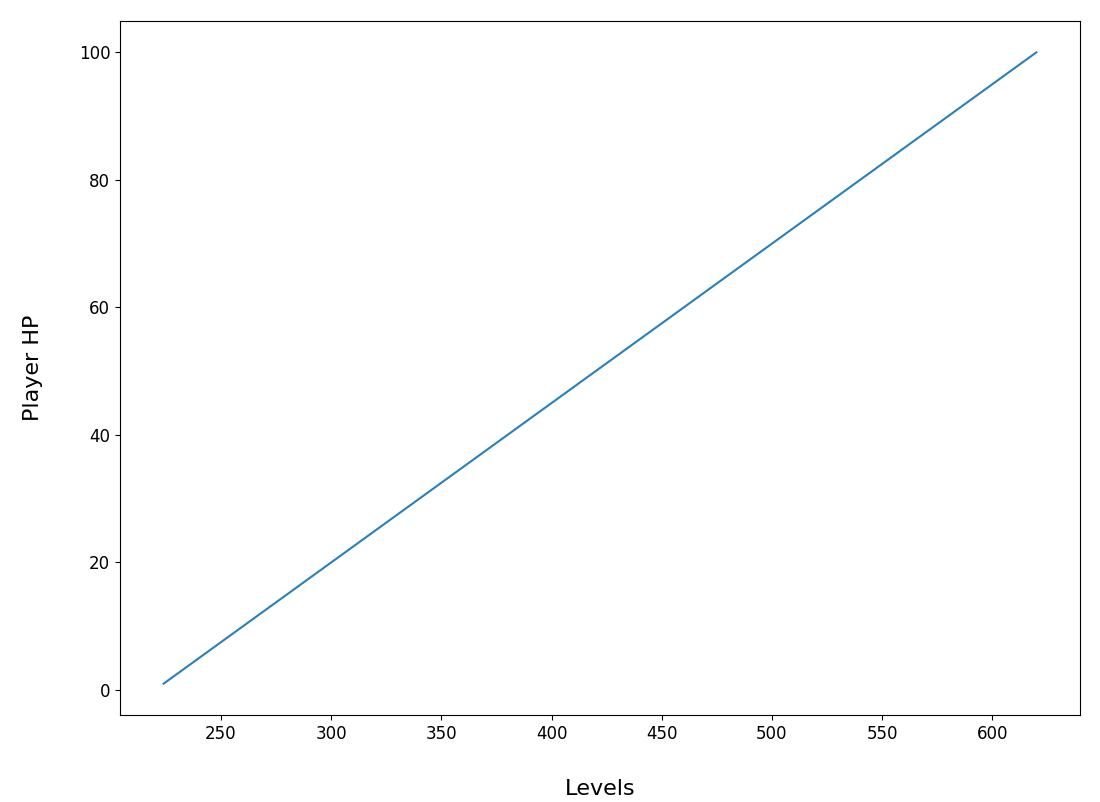
\includegraphics[scale=0.45]{img/PlayerHpDistrib1.png}
	\caption{Kenaikan HP setiap levelnya pada karakter pertama.}
	\label{fig:hp_player_1}
\end{figure}
\vspace{1ex}

\begin{figure} [!h] \centering
	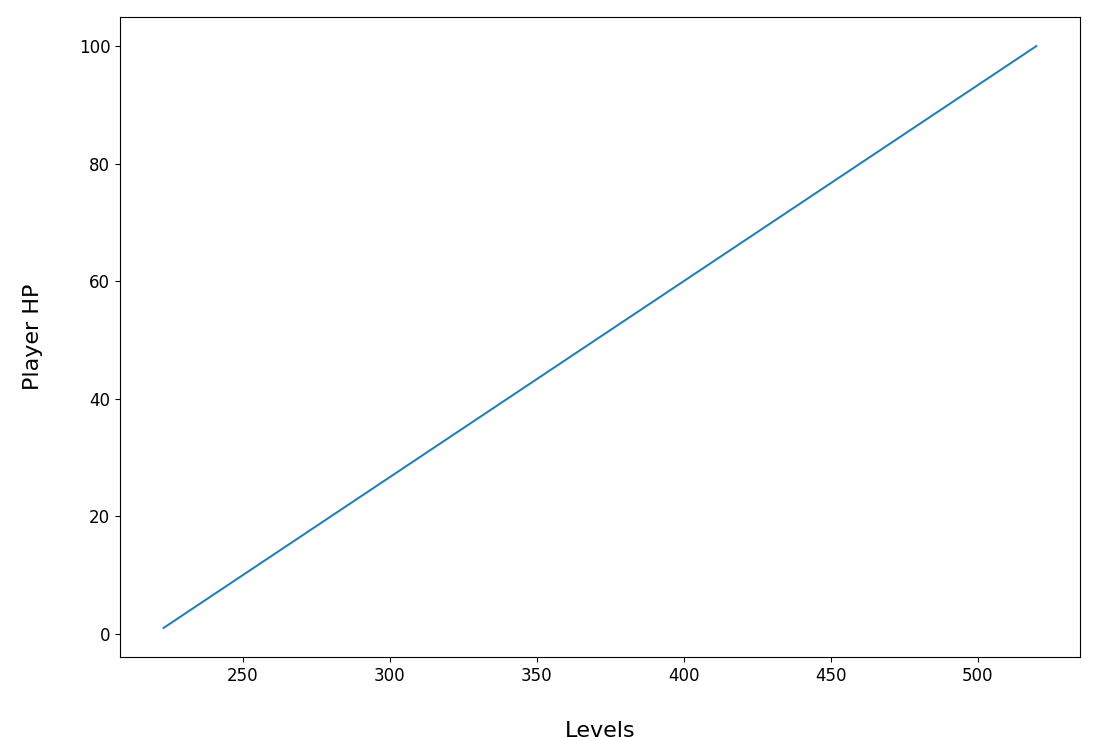
\includegraphics[scale=0.45]{img/PlayerHpDistrib2.png}
	\caption{Kenaikan HP setiap levelnya pada karakter kedua.}
	\vspace{1ex}
	\label{fig:hp_player_2}
\end{figure}

Sama seperti pada Gambar \ref{fig:mp_player_1} dan Gambar \ref{fig:mp_player_2} dengan jumlah MP dari pemain yang terus naik mengikuti pola yang dihasilkan pada Tabel \ref{tb:player_hp_mp_1} dan Tabel \ref{tb:player_hp_mp_2}, yang mana nilai tersebut diperoleh dari inisiasi variabel pada Tabel \ref{tb:player_input_variable} yaitu \textit{Max Level}, \textit{Start} MP dan \textit{Next} MP. Kemudian variabel-variabel tersebut dihitung dengan menggunakan persamaan \ref{eq:mp_player} agar membentuk pola kenaikan MP setiap levelnya seperti yang ditunjukan pada Gambar \ref{fig:mp_player_1} dan Gambar \ref{fig:mp_player_2}. 
\vspace{1ex}

\begin{figure} [!h] \centering
	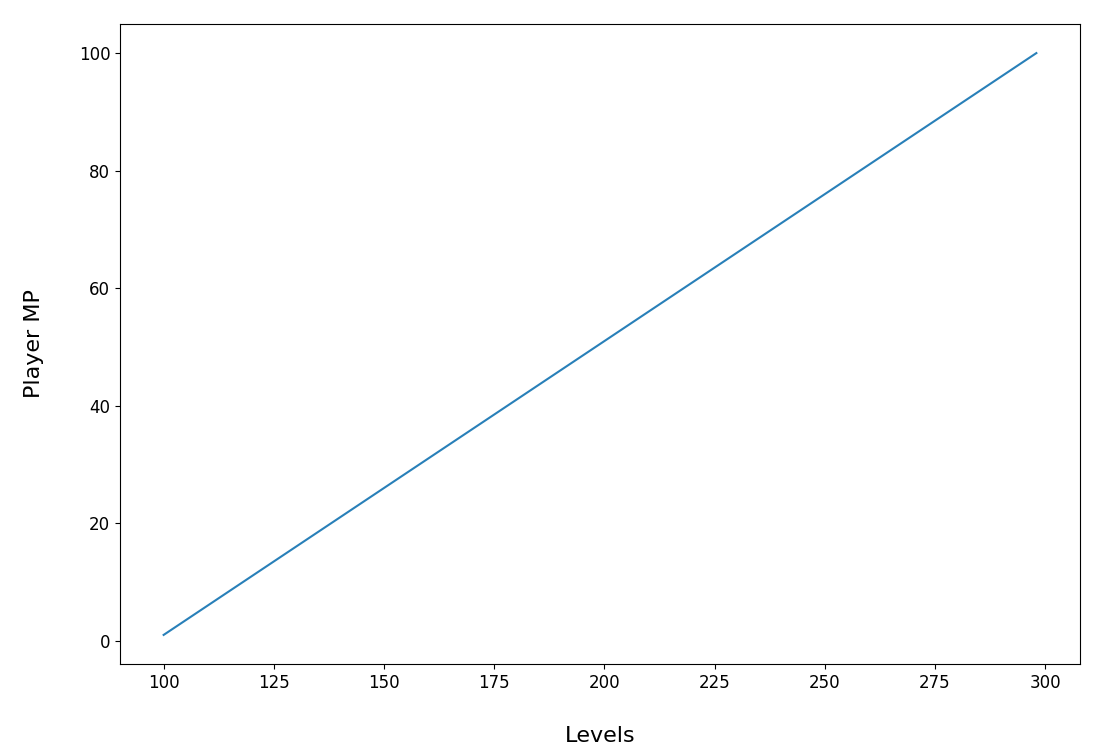
\includegraphics[scale=0.42]{img/PlayerMpDistrib1.png}
	\caption{Kenaikan MP setiap levelnya pada karakter pertama.}
	\label{fig:mp_player_1}
\end{figure}
\vspace{1ex}

\begin{figure} [!h] \centering
	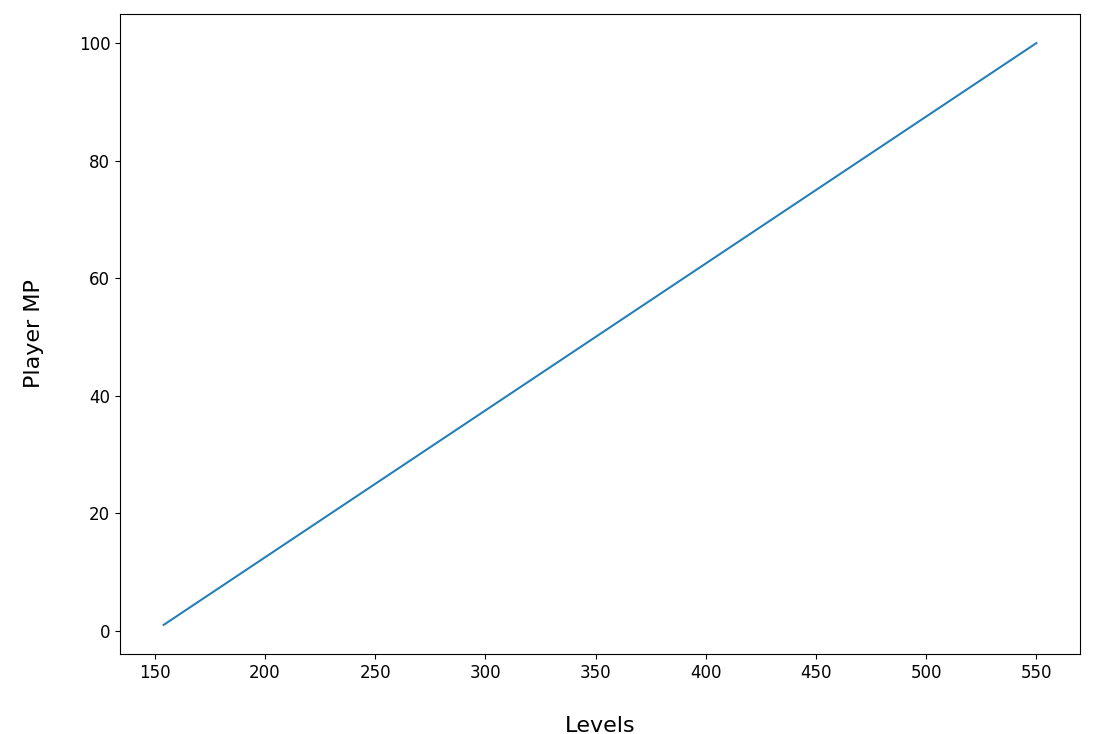
\includegraphics[scale=0.42]{img/PlayerMpDistrib2.png}
	\caption{Kenaikan MP setiap levelnya pada karakter kedua.}
	\label{fig:mp_player_2}
\end{figure}

Pada setiap proses pengujian dalam Sub-bab ini, yang dihasilkan pada Tabel \ref{tb:player_hp_mp_1} dan \ref{tb:player_hp_mp_2} menyajikan sebagian data saja. Hasil selengkapnya dapat dilihat pada Tabel \ref{tb:player_hp_mp_all_1} untuk karakter pertama dan pada \ref{tb:player_hp_mp_all_2} untuk karakter kedua yang terlampir dalam \nameref{chap:chap6_attachment}. Kemudian keseluruhan hasil tersebut divisualisasikan pada Gambar \ref{fig:hp_player_1}, dan Gambar \ref{fig:hp_player_2} untuk HP, Gambar \ref{fig:mp_player_1}, dan Gambar \ref{fig:mp_player_2} untuk MP.
\vspace{1ex}

\subsection{Distibusi Elemen dan Kelemahan Pemain}
\label{sec:sub_sec4_eval_dist_element_multi-character}
\vspace{1ex}

Sama seperti penjelasan pada Sub-bab \ref{sec:sub_sec4_eval_dist_element_single-character}, bila opsi distribusi elemen digunakan maka hasilnya akan tampak seperti pada Tabel \ref{tb:player_element_1} yang mengacu pada inputan dari Tabel \ref{tb:player_input_variable_eval_1} untuk karakter pemain pertama, sedangkan unt karakter pemain kedua hasilnya seperti pada Tabel \ref{tb:player_element_2} yang mengacu pada inputan dari Tabel \ref{tb:player_input_variable_eval_2}. Keduanya diasumsikan tidak adanya perubahan elemen dari karakter pemain dalam permainan.
\vspace{-1ex}

\begin{longtable}{|l|l|l|l|l|l|}
	\caption{Distribusi elemen pada karakter pemain pertama}
	\vspace{1ex}
	\label{tb:player_element_1}\\
	\hline
	\rowcolor[HTML]{C0C0C0} 
	\textbf{Phys} & \textbf{Water} & \textbf{Wind} & \textbf{Earth} & \textbf{Fire} \\ \hline
	0 & 0 & 2 & 1 & 0 \\ \hline
	0 & 0 & 2 & 1 & 0 \\ \hline
	0 & 0 & 2 & 1 & 0 \\ \hline
	0 & 0 & 2 & 1 & 0 \\ \hline
	0 & 0 & 2 & 1 & 0 \\ \hline
	0 & 0 & 2 & 1 & 0 \\ \hline
	... & ... & ... & ... & ... \\ \hline
	\textbf{0} & \textbf{0} & \textbf{2} & \textbf{1} & \textbf{0} \\ \hline
\end{longtable}
\vspace{-1ex}

\begin{longtable}{|l|l|l|l|l|l|}
	\caption{Distribusi elemen pada karakter pemain kedua}
	\vspace{1ex}
	\label{tb:player_element_2}\\
	\hline
	\rowcolor[HTML]{C0C0C0} 
	\textbf{Phys} & \textbf{Water} & \textbf{Wind} & \textbf{Earth} & \textbf{Fire} \\ \hline
	0 & 1 & 0 & 0 & 2 \\ \hline
	0 & 1 & 0 & 0 & 2 \\ \hline
	0 & 1 & 0 & 0 & 2 \\ \hline
	0 & 1 & 0 & 0 & 2 \\ \hline
	0 & 1 & 0 & 0 & 2 \\ \hline
	0 & 1 & 0 & 0 & 2 \\ \hline
	... & ... & ... & ... & ... \\ \hline
	\textbf{0} & \textbf{0} & \textbf{2} & \textbf{1} & \textbf{0} \\ \hline
\end{longtable}
\vspace{1ex}

Pada setiap proses pengujian dalam Sub-bab ini, yang dihasilkan pada Tabel \ref{tb:player_element_1} dan \ref{tb:player_element_2} menyajikan sebagian data saja. Hasil selengkapnya dapat dilihat pada Tabel \ref{tb:player_all_stats_1} sampai dengan Tabel \ref{tb:player_all_stats_4} dalam \nameref{chap:chap6_attachment}. Hal seperti penggunaan elemen pada pemain seperti pembahasan pada Sub-bab ini an sebelumnya, biasanya dijumpai pada permain RPG dengan Sub-genre JRPG, TRPG, WRPG dan MMORPG. Namun itu juga tidak semua permainan RPG dengan genre tersebut menggunakannya, hanya yang sering dijumpai saja.
\vspace{1ex}

\subsection{Pengujian Distibusi Stats Pemain}
\label{sec:sub_sec4_eval_multi-character_stats}
\vspace{1ex}

Pada bagian ini setiap langkah yang akan diuji sudah dijelaskan pada Sub-bab \ref{sec:sub_sec3_stat_pemain}, dimana pada bagian ini membahas tentang pembuatan \textit{stats} pemain untuk permaian RPG. Melalui berbagai proses seperti yang dijelaskan pada Sub-bab \ref{sec:sub_sec3_stat_pemain}, melalui data masukan pada Tabel \ref{tb:player_input_variable_eval_1} untuk karakter pertama dan Tabel \ref{tb:player_input_variable_eval_1} untuk karakter kedua, kemudian persamaan \ref{eq:KNN_bayes_player_stats} dan beberapa persamaan lain yang disebutkan pada Sub-bab \ref{sec:sub_sec3_stat_pemain} dihasilkan data seperti yang ditunjukan pada Tabel \ref{tb:player_battle_stats_1} dan \ref{tb:player_battle_stats_2}.
\vspace{-1ex}

\begin{longtable}{|l|l|l|l|l|l|}
	\caption{Distribusi \textit{stats} pada karakter pertama pemain}
	\vspace{1ex}
	\label{tb:player_battle_stats_1}\\
	\hline
	\rowcolor[HTML]{C0C0C0} 
	\textbf{Levels} & \textbf{Strength} & \textbf{Magic} & \textbf{Endurance} & \textbf{Speed} & \textbf{Luck} \\ \hline
	1 & 1 & 1 & 0 & 0 & 0 \\ \hline
	2 & 2 & 0 & 2 & 0 & 0 \\ \hline
	3 & 1 & 0 & 1 & 1 & 0 \\ \hline
	4 & 2 & 2 & 2 & 1 & 0 \\ \hline
	5 & 0 & 0 & 0 & 0 & 0 \\ \hline
	6 & 2 & 0 & 0 & 1 & 0 \\ \hline
	7 & 0 & 0 & 0 & 1 & 0 \\ \hline
	8 & 0 & 0 & 0 & 0 & 0 \\ \hline
	... & ... & ... & ... & ... & ... \\ \hline
	\textbf{100} & \textbf{74} & \textbf{38} & \textbf{63} & \textbf{65} & \textbf{60} \\ \hline
\end{longtable}

\begin{longtable}{|l|l|l|l|l|l|}
	\caption{Distribusi stats pada karakter pemain}
	\vspace{1ex}
	\label{tb:player_battle_stats_2}\\
	\hline
	\rowcolor[HTML]{C0C0C0} 
	\textbf{Levels} & \textbf{Strength} & \textbf{Magic} & \textbf{Endurance} & \textbf{Speed} & \textbf{Luck} \\ \hline
	1 & 1 & 2 & 0 & 0 & 1 \\ \hline
	2 & 0 & 2 & 0 & 2 & 0 \\ \hline
	3 & 1 & 0 & 0 & 0 & 0 \\ \hline
	4 & 1 & 1 & 0 & 0 & 0 \\ \hline
	5 & 1 & 1 & 0 & 0 & 0 \\ \hline
	6 & 1 & 1 & 0 & 2 & 1 \\ \hline
	7 & 0 & 0 & 0 & 0 & 1 \\ \hline
	... & ... & ... & ... & ... & ... \\ \hline
	\textbf{100} & \textbf{60} & \textbf{68} & \textbf{57} & \textbf{58} & \textbf{57} \\ \hline
\end{longtable}
\vspace{1ex}

Pada Tabel \ref{tb:player_battle_stats_1} dan \ref{tb:player_battle_stats_2} yang masing-masing adalah data \textit{stats} dari karakter pemain pertama dan kedua yang dihasilakn melalui penambahan nilai pada \textit{stats} secara acak pada setiap \textit{stats}. Seperti yang dijelaskan pada persaamaan \ref{eq:nbayes_class}, \ref{eq:KNN_distance_stats}, dan persamaan \ref{eq:KNN_bayes_player_stats} saat nilai \textit{stats} di tambahkan secara acak dari 1 sampai dengan 2 pada level yang berjarak antara 1 sampai dengan 100. Selanjutnya representasi dari hasil penambahan \textit{stats} tersebut yang ditunjukan melalui Gambar \ref{fig:stats_player_1} dan Gambar \ref{fig:stats_player_2} yang masing-masing adalah karakter pertama dan kedua dari pemain secara berurutan, nilai dari setiap \textit{stats} pada masing-masing karakter terus naik sesuai dengan level dari masing-masing karakter yang juga terus naik. 
\vspace{1ex}

\begin{figure} [!h] \centering
	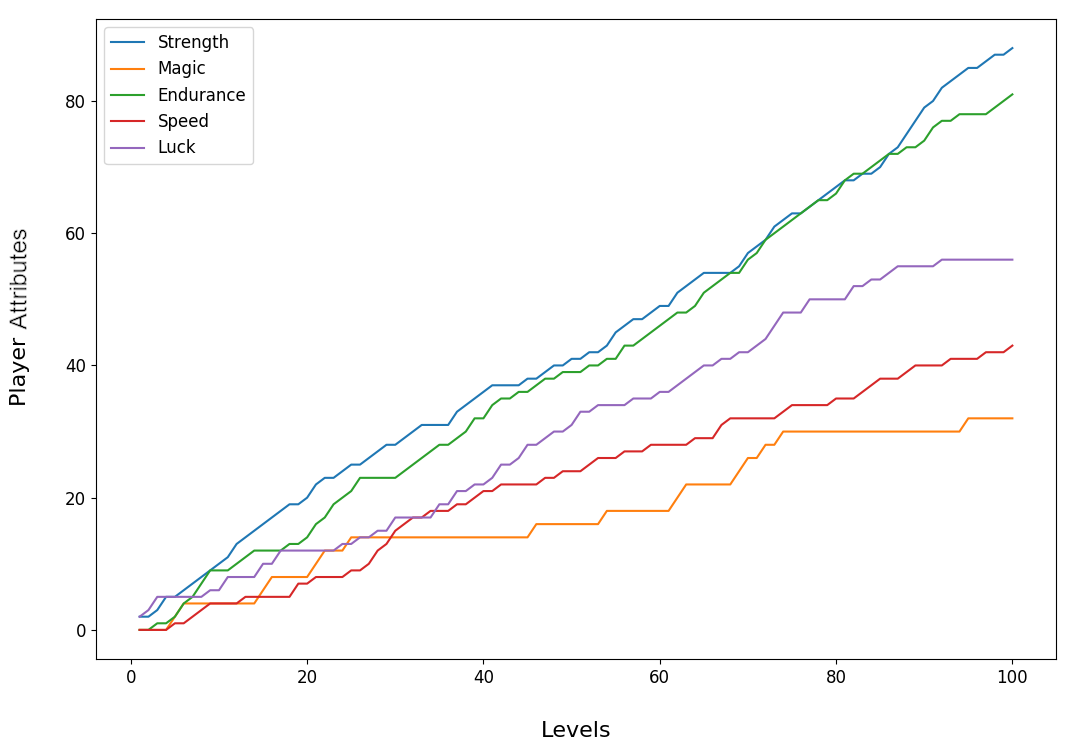
\includegraphics[scale=0.52]{img/PlayerStatsDistrib1.png}
	\caption{Kenaikan stats karakter pertama dari pemain setiap levelnya.}
	\label{fig:stats_player_1}
\end{figure}

\begin{figure} [!h] \centering
	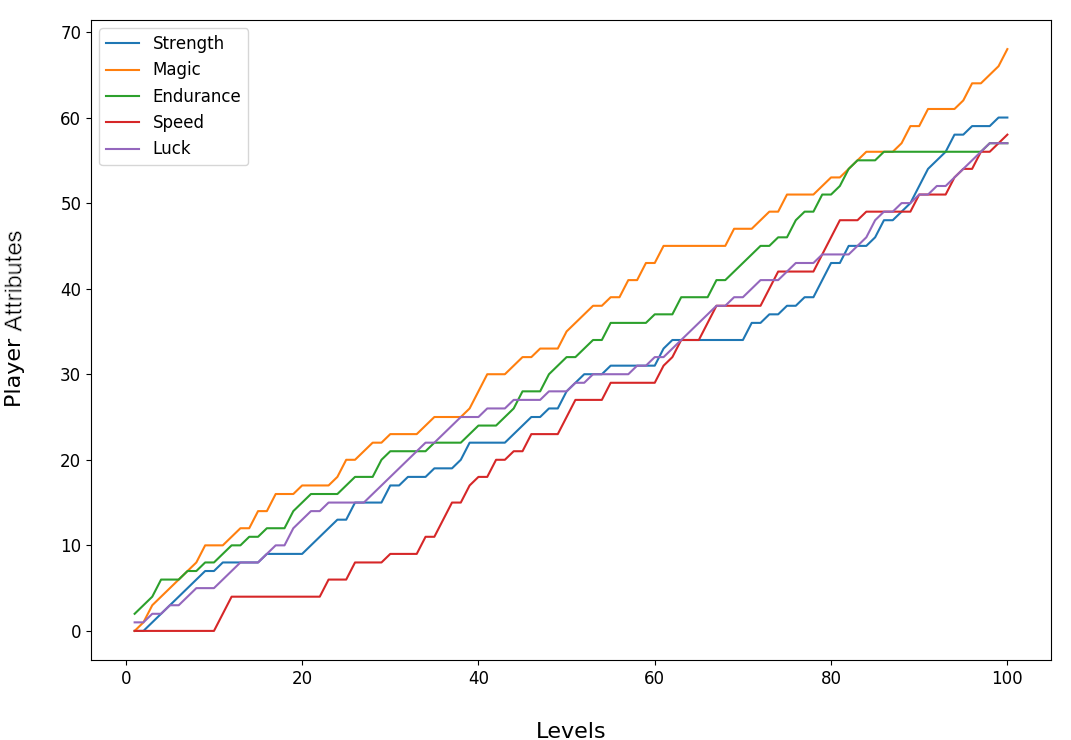
\includegraphics[scale=0.52]{img/PlayerStatsDistrib2.png}
	\caption{Kenaikan stats karakter kedua dari pemain setiap levelnya.}
	\label{fig:stats_player_2}
\end{figure}

Pada setiap proses pengujian dalam Sub-bab ini, yang dihasilkan pada Tabel \ref{tb:player_battle_stats} menyajikan sebagian data saja. Hasil selengkapnya dapat dilihat pada Tabel \ref{tb:player_all_stats_1} sampai dengan Tabel \ref{tb:player_all_stats_4} dalam \nameref{chap:chap6_attachment} yang keseluruhan hasil tersebut divisualisasikan pada Gambar \ref{fig:stats_player_1} dan Gambar \ref{fig:stats_player_1}.
\vspace{1ex}

\section{Pembuatan Stats Musuh}
\label{sec:sec4_eval_turn-based_enemy}
\vspace{1ex}

Pada bagian ini setiap langkah yang akan diuji sudah dijelaskan pada Bagian \ref{sec:sec3_enemy_stats}, dimana pada bagian ini membahas tentang pembuatan \textit{stats} musuh untuk permaian dengan genre RPG. Melalui berbagai proses seperti yang dijelaskan pada Bagian \ref{sec:sec3_player_stats}, maka pada beberapa Sub-bab dibawah ini adalah langkah-langkah dalam proses pengujiannya.
\vspace{1ex}


\subsection{Distibusi Level Musuh}
\label{sec:sub_sec4_eval_dist_enemy_level}
\vspace{1ex}

Seperti yang sudah dijelaskan pada Sub-bab \ref{sec:sub_sec3_enemy_level}, dimana pada bagian ini membahas tentang pendistribusian level musuh untuk permaian dengan genre RPG. Berikut adalah hasil dari proses distribusi level yang diperoleh dari perhitungan pada persamaan \ref{eq:enemy_levels1}, \ref{eq:enemy_levels2}, \ref{eq:sub_enemy_levels1}, \ref{eq:sub_enemy_levels2} dan persamaan \ref{eq:probability_enemy_levels}. Setelah melalui tahapan tersebut dan dengan variabel masukan pada Tabel \ref{tb:enemy_input_variable} maka level yang dihasilkan akan seperti pada Tabel \ref{tb:enemy_level_distrib}.
\vspace{-1ex}

\begin{longtable}{|l|l|l|}
	\caption{Hasil level yang dibuat untuk musuh.}
	\label{tb:enemy_level_distrib}\\
	\hline
	\rowcolor[HTML]{C0C0C0} 
	\textbf{No.} & \textbf{Name} & \textbf{Levels} \\ \hline
	1 & Enemy 1 & 1 \\ \hline
	2 & Enemy 2 & 1 \\ \hline
	3 & Enemy 3 & 1 \\ \hline
	4 & Enemy 4 & 1 \\ \hline
	5 & Enemy 5 & 2 \\ \hline
	6 & Enemy 6 & 2 \\ \hline
	7 & Enemy 7 & 2 \\ \hline
	8 & Enemy 8 & 2 \\ \hline
	9 & Enemy 9 & 2 \\ \hline
	10 & Enemy 10 & 2 \\ \hline
	11 & Enemy 11 & 2 \\ \hline
	12 & Enemy 12 & 2 \\ \hline
	13 & Enemy 13 & 2 \\ \hline
	14 & Enemy 14 & 3 \\ \hline
	15 & Enemy 15 & 3 \\ \hline
	... & ... & ... \\ \hline
	\textbf{400} & \textbf{Enemy 400} & \textbf{78} \\ \hline
\end{longtable}
\vspace{1ex}

Pada Tabel \ref{tb:enemy_level_distrib} adalah sebagian data dari level yang dihasilkan oleh program, untuk hasil lebih lengkapnya bisa dilihat pada Tabel \ref{tb:enemies_all_stats_1} sampai Tabel \ref{tb:enemies_all_stats_15} dalam BAB \nameref{chap:chap6_attachment} pada Tabel \ref{tb:enemies_all_stats_1} sampai dengan Tabel \ref{tb:enemies_all_stats_15} di kolom \textit{Levels}. Kemudian persebaran level yang dihasilkan tersebut bila divisualisasikan maka hasilnya akan seperti yang ditujukkkan pada Gambar \ref{fig:enemy_level_distrib}. Grafik atau histogram yang ditunjukan pada Gambar \ref{fig:enemy_level_distrib} tersebut sangatlah tidak merata, hal tersebut dikarenakan proses penentuan level yang ditentukan secara acak.

\begin{figure} [!h] \centering
	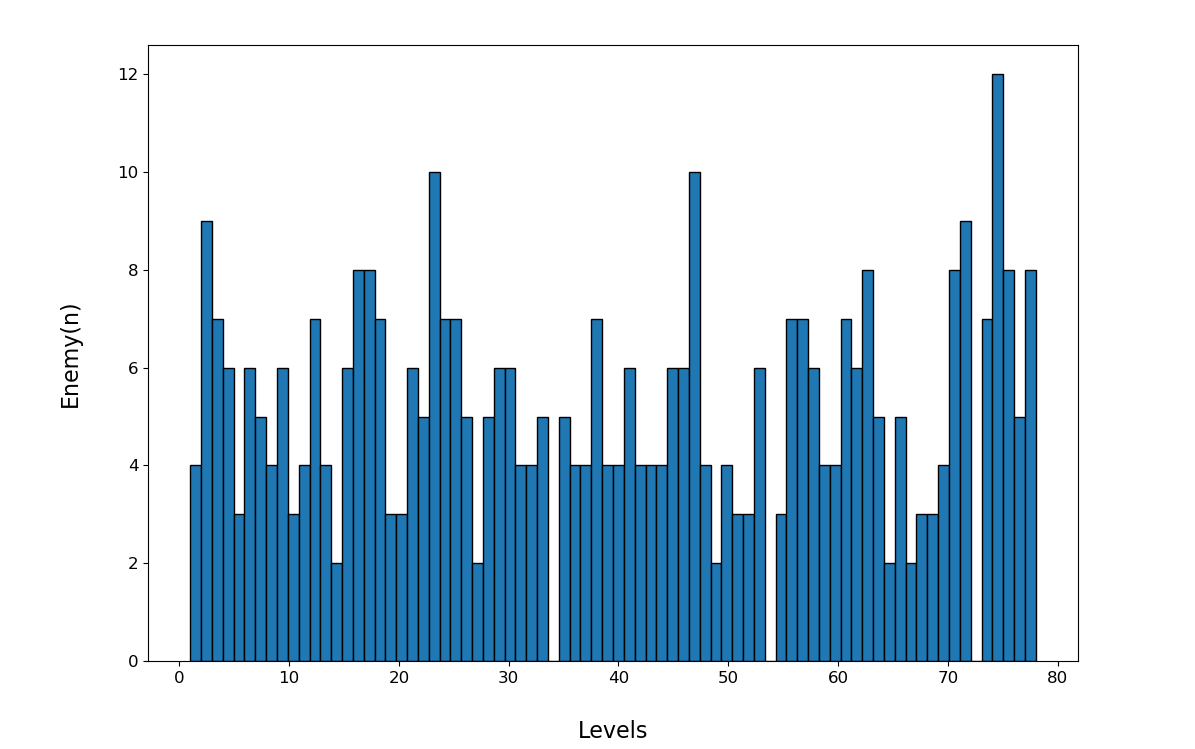
\includegraphics[scale=0.45]{img/EnemyLevelDistrib.png}
	\caption{Distribusi Level Musuh.}
	\label{fig:enemy_level_distrib}
\end{figure}

Di lanjutkan dengan validasi dari keseimbangan persebaran level musuh, hal ini dilakukan dengan menggunakkan persamaan melalui beberapa langkah seperti yang ditunjukan oleh persamaan \ref{eq:mean_enemy_levels}, \ref{eq:varian_enemy_levels}, \ref{eq:stdev_enemy_levels} dan persamaan \ref{eq:PDF_enemy_levels}. Konsep tersebut beracuan pada Sub-bab \ref{sec:sub_sec2_gauss_bayes} tentang \textit{Gaussian Naive bayes}, dengan harapan apakah setiap data yang dihasilkan sebelumnya sudah terdistribusi dengan normal atau tidak. Jika memang benar data hasil program ini valid maka ketika musuh bertambah maka pola dari level dan jumlah musuh masih akan membentuk pola distribusi normal seperti pada Gambar \ref{fig:enemy_level_distrib_ndist}.
\vspace{1ex}

\begin{figure} [!h] \centering
	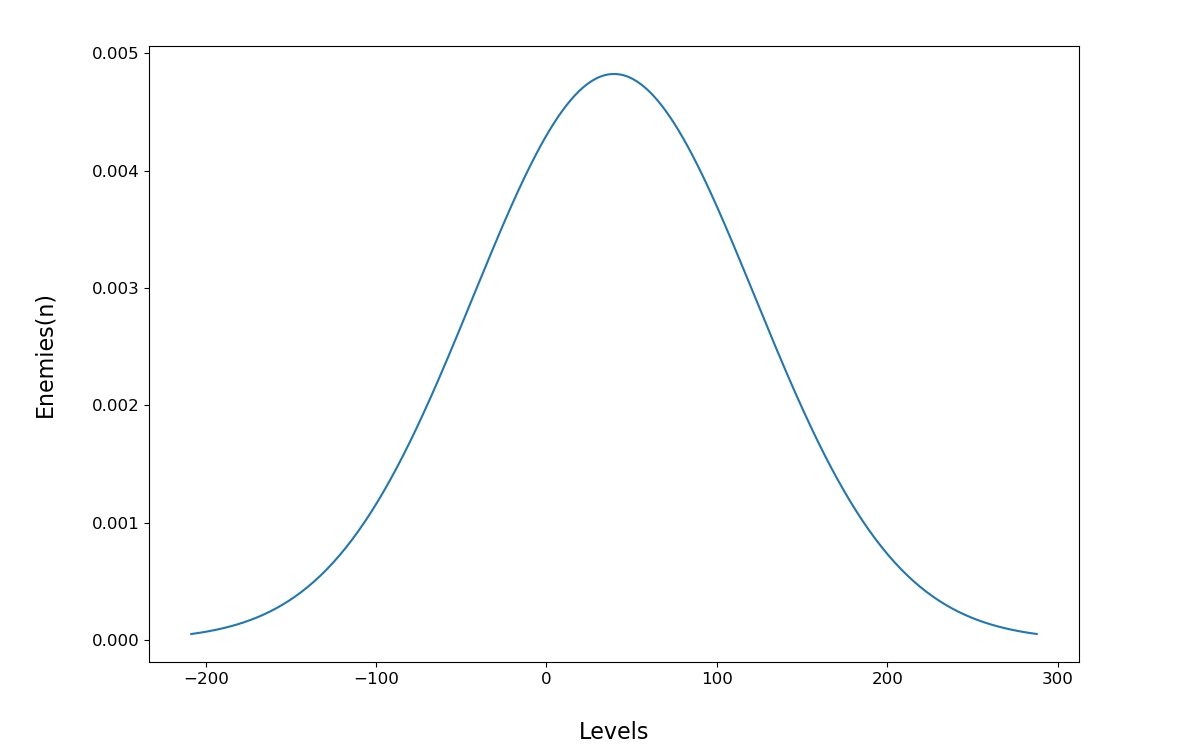
\includegraphics[scale=0.45]{img/EnemyLevelDistribNdist.png}
	\caption{Distribusi level musuh dalam bentuk distribusi normal.}
	\label{fig:enemy_level_distrib_ndist}
\end{figure}

Pada Gambar \ref{fig:enemy_level_distrib_ndist} jika dilihat persebaran datanya dari kiri ke kanan menggambarkan tingkat kesulitan musuh berdasarkan level, jumlah musuh pada sisi kiri berjumlah sedikit semakin ke kanan jumlahnya meningkat dan semakin ke kanan jumlah musuh kembali menjadi sedikit jumlahnya. Hal tersebut menggambarkan tingkat keseimbangan dari musuh yang dibuat, yang mana jumlah musuh dengan level menengah berjumlah paling banyak dan jumlah musuh yang sangat sulit dan sangat mudah dikalahkan berjummlah sedikit. Tujuan utama dari kondisi tersebut adalah terjadinya keseimbangan saat terjadinya pertarungan antara pemain dan musuh.
\vspace{1ex}


\subsection{Distibusi Type Musuh}
\label{sec:sub_sec4_eval_dist_enemy_type}
\vspace{1ex}

Seperti yang sudah dijelaskan pada Sub-bab \ref{sec:sub_sec3_enemy_type}, dimana pada bagian ini membahas tentang pendistribusian tipe musuh untuk permaian dengan genre \textit{turn-based} RPG. Berikut adalah hasil dari proses distribusi tipe musuh yang diperoleh dari perhitungan pada persamaan \ref{eq:enemy_types_percentage}, \ref{eq:enemy_types_dist_level}, \ref{eq:enemy_types_rest_dist_level}, \ref{eq:enemy_types_probability}, \ref{eq:enemy_rest_types} dan persamaan \ref{eq:enemy_types_rest_probability}. Setelah melalui tahapan tersebut dengan variabel masukan pada Tabel \ref{tb:enemy_input_variable} maka hasil distribusi dan penjelasan level yang dilakukan oleh beberapa persamaan tersebut akan menjadi seperti Tabel \ref{tb:enemy_type_distrib}.

\begin{longtable}{|l|l|l|l|}
	\caption{Hasil level yang dibuat untuk musuh.}
	\label{tb:enemy_type_distrib}\\
	\hline
	\rowcolor[HTML]{C0C0C0} 
	\textbf{No.} & \textbf{Name} & \textbf{Levels} & \textbf{Type} \\ \hline
	1 & Enemy 1 & 1 & 0 \\ \hline
	2 & Enemy 2 & 1 & 0 \\ \hline
	3 & Enemy 3 & 1 & 2 \\ \hline
	4 & Enemy 4 & 1 & 1 \\ \hline
	5 & Enemy 5 & 2 & 2 \\ \hline
	6 & Enemy 6 & 2 & 1 \\ \hline
	7 & Enemy 7 & 2 & 2 \\ \hline
	8 & Enemy 8 & 2 & 0 \\ \hline
	9 & Enemy 9 & 2 & 2 \\ \hline
	10 & Enemy 10 & 2 & 2 \\ \hline
	11 & Enemy 11 & 2 & 4 \\ \hline
	12 & Enemy 12 & 2 & 0 \\ \hline
	13 & Enemy 13 & 2 & 0 \\ \hline
	14 & Enemy 14 & 3 & 4 \\ \hline
	15 & Enemy 15 & 3 & 4 \\ \hline
	16 & Enemy 16 & 3 & 2 \\ \hline
	... & ... & ... & ... \\ \hline
	\textbf{400} & \textbf{Enemy 400} & \textbf{78} & \textbf{3} \\ \hline
\end{longtable}

Dari data yang tedapat pada Tabel \ref{tb:enemy_type_distrib} hanya sebagian data saja, lebih lengkapnya dapat dilihat langsung pada \nameref{chap:chap6_attachment} dalam Tabel \ref{tb:enemies_all_stats_1} sampai dengan Tabel \ref{tb:enemies_all_stats_15} di kolom \textit{Type}. Pada Tabel \ref{tb:enemy_type_distrib} dan tabel lain yang memuat tentang \textit{Type} yang berisi data $ET_{i}$ atau jenis musuh yang diisi dengan angka 0 sampai dengan 4, maksud dari angka tersebut adalah untuk mewakili indeks dari variabel \textit{Enemy Type} pada Tabel \ref{tb:enemy_input_variable}. Secara berurutan dari 0 sampai dengan 4 adalah \textit{Mixed}, \textit{Hard Magic}, \textit{Soft Magic}, \textit{Hard Strength}, dan \textit{Soft Magic}. Seluruh data tersebut jika divisualisasikan maka hasilnya seperti Gambar \ref{fig:enemy_type_distrib} sesuai yang ditargetkan oleh variabel \textit{Distribute Percentage} pada Tabel \ref{tb:enemy_input_variable} atau variabel $DP$ pada persamaan \ref{eq:enemy_types_percentage}.

\begin{figure} [!h] \centering
	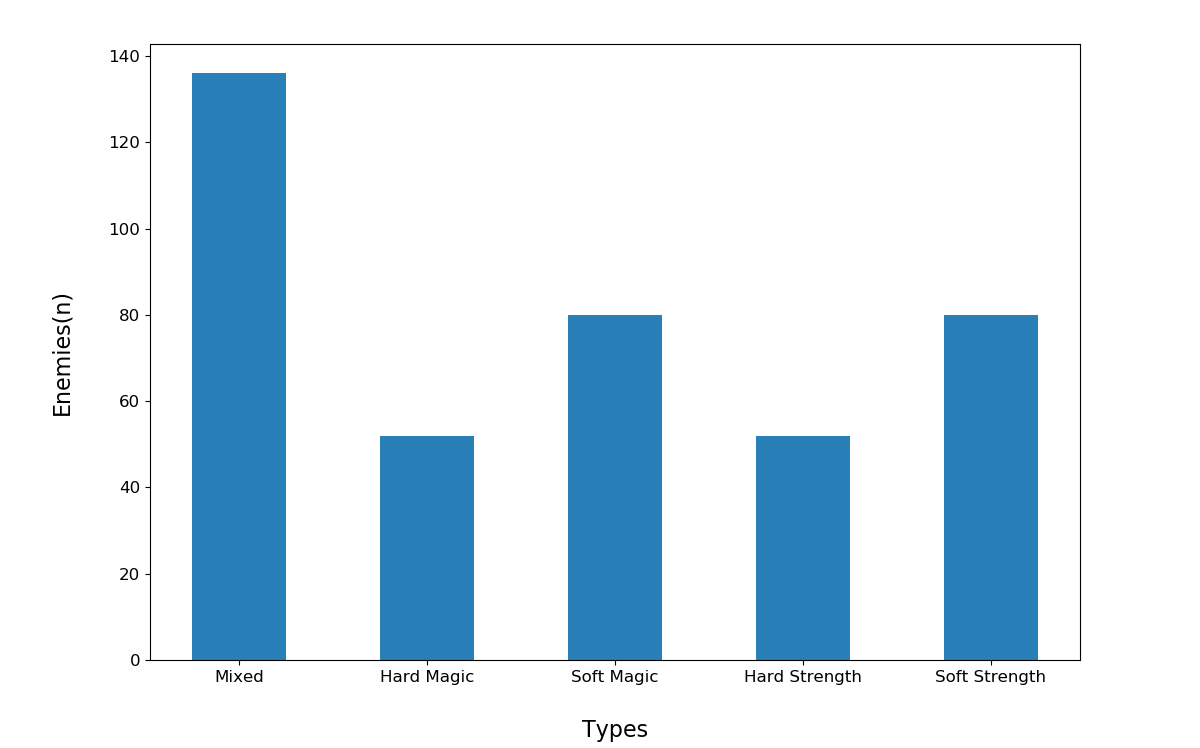
\includegraphics[scale=0.5]{img/EnemyTypeDistrib.png}
	\caption{Distribusi tipe musuh.}
	\label{fig:enemy_type_distrib}
\end{figure}

Kemudian pada Gambar \ref{fig:enemy_type_distrib} adalah hasil dari proses pembuatan dan pengelompokan musuh berdasarkan tipe yang sudah sesuai dengan variabel masukan pada Tabel \ref{tb:enemy_input_variable}. Dengan musuh bertipe \textit{Mixed} berjumlah yang paling banyak, diikuti \textit{soft magic} dan \textit{soft strength} dengan harapan bahwa ini adalah musuh yang memiliki karakter \textit{magic} dan \textit{strength} namun masih mudah dikalahkan, dilanjutkan dengan yang paling sedikit adalah \textit{hard magic} dan \textit{hard strength} dengan harapan menjadi musuh berkarakter strength dan magic yang sulit dikalahkan.
\vspace{1ex}

\subsection{Distribusi Element dan Kelemahan pada Musuh}
\label{sec:sub_sec4_eval_dist_enemy_element_and_weak}
\vspace{1ex}

Seperti yang sudah dijelaskan pada Sub-bab \ref{sec:sub_sec3_enemy_weak}, dimana pada bagian ini membahas tentang pendistribusian elemen dan kelemahan musuh untuk permaian dengan genre \textit{turn-based} RPG. Berikut adalah hasil dari proses distribusi tipe musuh yang diperoleh dari perhitungan pada persamaan \ref{eq:enemy_element}, \ref{eq:damage_name_number}, \ref{eq:damage_number_prob}, \ref{eq:multi_damage_num_prob}, dan \ref{eq:all_enemies_damage}. Setelah melalui tahapan tersebut dengan variabel masukan pada Tabel \ref{tb:enemy_input_variable} maka hasil persebaran kelemahan dan kekebalan musuh ditunjukkan pada Tabel \ref{tb:enemy_weak_distrib} dan selengkapnya dapat dilihat pada \nameref{chap:chap6_attachment} dalam Tabel \ref{tb:enemies_all_stats_1} sampai dengan Tabel \ref{tb:enemies_all_stats_15}.
\vspace{-1ex}

\begin{longtable}{|l|l|l|l|l|l|l|}
	\caption{Hasil level yang dibuat untuk musuh.}
	\label{tb:enemy_weak_distrib}\\
	\hline
	\rowcolor[HTML]{C0C0C0} 
	\textbf{No.} & \textbf{Name} & \textbf{Phys} & \textbf{Water} & \textbf{Wind} & \textbf{Earth} & \textbf{Fire} \\ \hline
	1 & Enemy 1 & 1 & 1 & 0 & 1 & 0 \\ \hline
	2 & Enemy 2 & 0 & 0 & 0 & 0 & 0 \\ \hline
	3 & Enemy 3 & 0 & 1 & 0 & 1 & 1 \\ \hline
	4 & Enemy 4 & 1 & 0 & 1 & 0 & 0 \\ \hline
	5 & Enemy 5 & 0 & 1 & 0 & 0 & 1 \\ \hline
	6 & Enemy 6 & 1 & 1 & 0 & 1 & 0 \\ \hline
	7 & Enemy 7 & 1 & 0 & 0 & 0 & 0 \\ \hline
	8 & Enemy 8 & 0 & 0 & 0 & 0 & 1 \\ \hline
	9 & Enemy 9 & 1 & 1 & 0 & 0 & 0 \\ \hline
	10 & Enemy 10 & 0 & 0 & 0 & 0 & 0 \\ \hline
	11 & Enemy 11 & 1 & 0 & 0 & 1 & 0 \\ \hline
	12 & Enemy 12 & 0 & 0 & 0 & 0 & 1 \\ \hline
	13 & Enemy 13 & 0 & 0 & 2 & 1 & 0 \\ \hline
	%14 & Enemy 14 & 0 & 1 & 0 & 0 & 0 \\ \hline
	... & ... & ... & ... & ... & ... & ... \\ \hline
	\textbf{400} & \textbf{Enemy 400} & \textbf{0} & \textbf{0} & \textbf{2} & \textbf{1} & \textbf{0} \\ \hline
\end{longtable}
\vspace{1ex}

Jika melihat Tabel \ref{tb:enemy_weak_distrib} dengan melihat pada kolom \textit{Phys}, \textit{Water}, \textit{Wind}, \textit{Earth}, dan \textit{Fire}, isi dari kolom tersebut berupa angka nol sampai dengan dua adalah hasil dari pembuatan \textit{stats} kelemahan musuh pada variabel $DmgEN_{M}$ atau untuk $DmgEN_{M} = \left \{ DmgNu_{0}, DmgNu_{1}, DmgNu_{2},..., DmgNu_{M} \right \}$ jika jumlah kelemahan musuh lebih dari tiga atau yang dicontohkan pada Tabel \ref{tb:enemy_input_variable} dalam variabel \textit{List Damage}. Hasil dari proses yang sebelumnya dijelaskan pada Sub-bab ini menghasilkan persebaran kelemahan dan kekebalan musuh yang ditunjukkan pada Gambar \ref{fig:enemy_weak_distrib} dibawah ini.

\begin{figure} [!h] \centering
	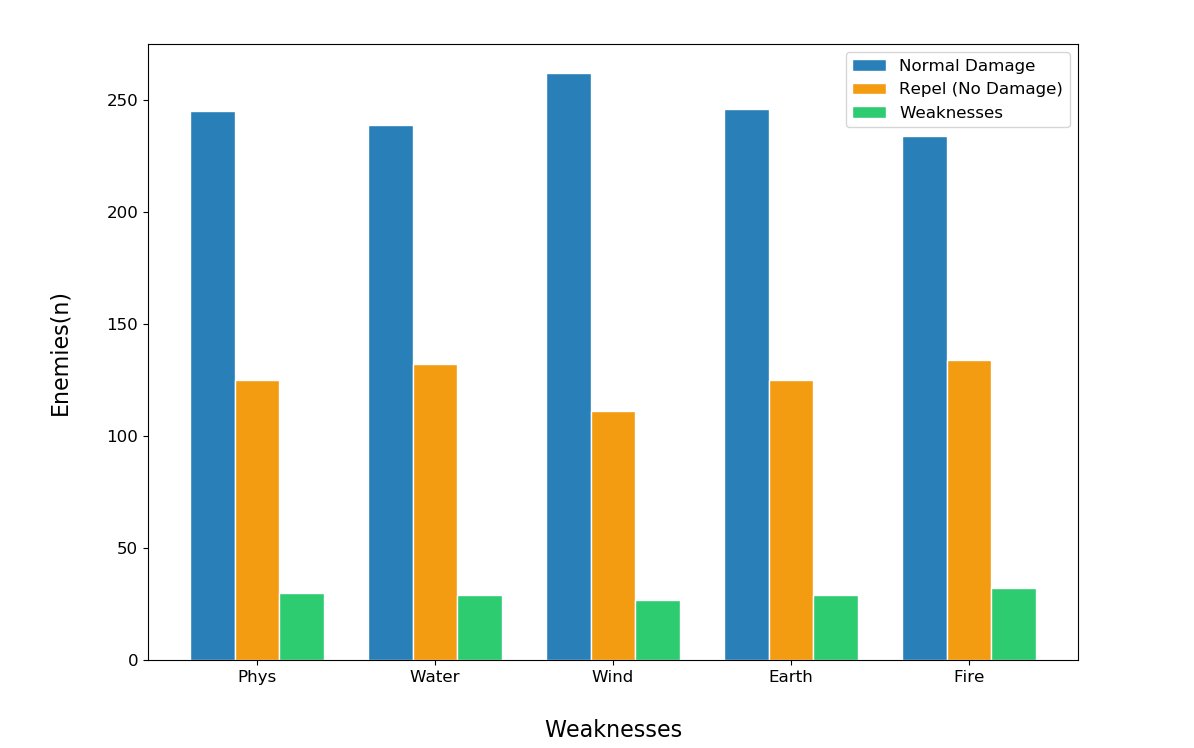
\includegraphics[scale=0.50]{img/EnemyWeakDistrib.png}
	\caption{Distribusi kelemahan musuh.}
	\label{fig:enemy_weak_distrib}
\end{figure}

Pada Gambar \ref{fig:enemy_weak_distrib} dapat dilihat distribusi musuh dengan kelemahan dan kekebalannya. Terlihat pada kondisi tersebut jumlah musuh dengan kondisi \textit{Normal} memiliki nilai paling tunggi pada setiap kelemahan, hal tersebut dapat diartikan bahwa sebagian besar elemen dari musuh dapat memperoleh \textit{damage} secara normal jika diserang. Kemudian jumlah musuh pada kondisi \textit{Repel} berjumlah terbanyak kedua, hal tersebut dapat diartikan musuh memmiliki jumlah kekebalan terhadap serangan sejumlah angka pada setiap elemen pada Gambar \ref{fig:enemy_weak_distrib}. Begitu juga dengan kondisi \textit{Weaknesses} dengan jumlah paling sedikit, hal tersebut bertujuan agar menjadikan pertarungan antara pemain dan musuh menjadi tidak mudah dimenangkan oleh pemain. Tidak hanya dengan efek \textit{Weaknesses}, efek \textit{Repel} juga sangat berpengaruh dalam menjadikan permainan seperti layaknya sebuah \textit{puzzle} atau teka-teki.
\vspace{1ex}

Sedangkan pada persamaan \ref{eq:multi_damage_num_prob} adalah penjelasan tentang proses munculnya setiap $DmgNu$ pada satu karakter musuh, sehingga variabel tersebut berubah menjadi $DmgNu_{i}$. Seperti penjelasan sebelumnya bahwa pada sebuah karakter musuh dapat memiliki lebih dari satu kelemahan atau kekebalan $DmgNu$ terhadap $DmgNa$ yang diset secara acak seperti yang sudah dijelaskan pada bagian sebelumnya. 
\vspace{1ex}


\subsection{Distribusi HP, MP, dan Stats Musuh}
\label{sec:sub_sec4_eval_dist_enemy_HP_MP_Stats}
\vspace{1ex}

pada Sub-bab \ref{sec:sub_sec3_enemy_hp_mp_stats}, dimana pada bagian ini membahas tentang pendistribusian HP dan MP musuh untuk permaian dengan genre \textit{turn-based} RPG. Berikut adalah hasil dari proses distribusi tipe musuh yang diperoleh dari perhitungan pada persamaan \ref{eq:enemy_types_stats_ex} sampai dengan persamaan \ref{eq:enemy_types_prob_hp_mix}, yang mana pada persamaan \ref{eq:enemy_types_stats_ex} sampai dengan persamaan \ref{eq:enemy_types_prob_adv} adalah penenentuan tipe musuh. Setelah melalui tahapan tersebut dengan variabel masukan pada Tabel \ref{tb:enemy_input_variable} maka hasil persebaran kelemahan dan kekebalan musuh ditunjukkan pada Tabel \ref{tb:enemy_weak_distrib}.
\vspace{-1ex}

\begin{longtable}{|l|l|l|l|l|}
	\caption{Distribusi \textit{Stats} HP dan MP musuh.}
	\label{tb:enemy_weak_stats}\\
	\hline
	\rowcolor[HTML]{C0C0C0} 
	\textbf{No.} & \textbf{Name} & \textbf{Levels} & \textbf{HP} & \textbf{MP} \\ \hline
	1 & Enemy 1 & 1 & 42 & 45 \\ \hline
	2 & Enemy 2 & 1 & 84 & 21 \\ \hline
	3 & Enemy 3 & 1 & 43 & 51 \\ \hline
	4 & Enemy 4 & 1 & 44 & 231 \\ \hline
	5 & Enemy 5 & 2 & 40 & 40 \\ \hline
	6 & Enemy 6 & 2 & 44 & 208 \\ \hline
	7 & Enemy 7 & 2 & 44 & 47 \\ \hline
	8 & Enemy 8 & 2 & 42 & 53 \\ \hline
	9 & Enemy 9 & 2 & 49 & 53 \\ \hline
	10 & Enemy 10 & 2 & 42 & 49 \\ \hline
	11 & Enemy 11 & 2 & 44 & 23 \\ \hline
	12 & Enemy 12 & 2 & 79 & 27 \\ \hline
	13 & Enemy 13 & 2 & 41 & 26 \\ \hline
	14 & Enemy 14 & 3 & 50 & 34 \\ \hline
	15 & Enemy 15 & 3 & 54 & 20 \\ \hline
	... & ... & ... & ... & ... \\ \hline
	\textbf{400} & \textbf{Enemy 400} & \textbf{78} & \textbf{389} & \textbf{161} \\ \hline
\end{longtable}
\vspace{1ex}

Pada Tabel \ref{tb:enemy_weak_stats} hanya sebagian data saja yang ditampilkan, untuk selengkapnya dapat dilihat pada \nameref{chap:chap6_attachment} dalam Tabel \ref{tb:enemies_all_stats_1} sampai dengan Tabel \ref{tb:enemies_all_stats_15} pada kolom HP dan MP. Selanjutnya adalah penggambaran persebaran \textit{stats} HP dan MP yang masing-masing digambarkan pada Gambar \ref{fig:enemy_hp_distrib} dan Gambar \ref{fig:enemy_mp_distrib}.
\vspace{1ex}

\begin{figure} [!h] \centering
	\centering
	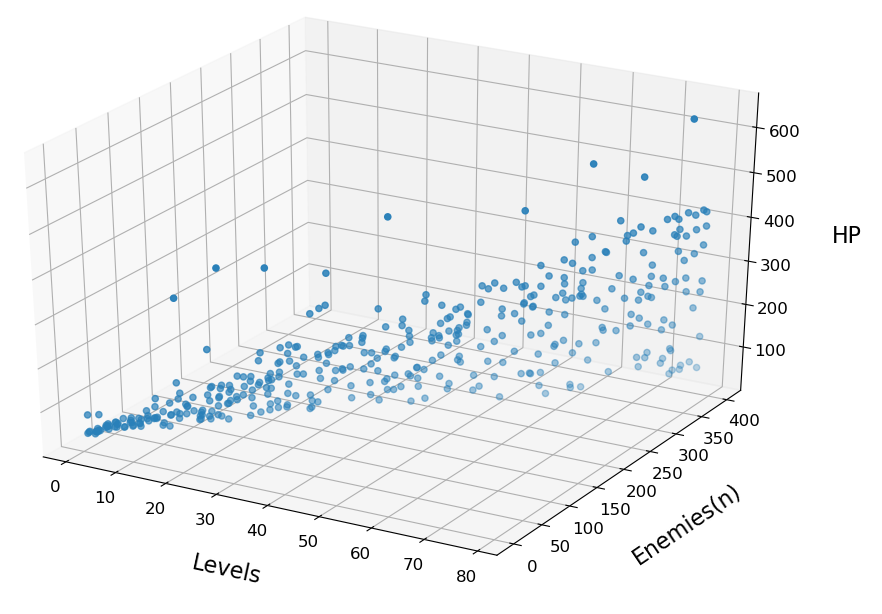
\includegraphics[scale=0.57]{img/EnemyHpDistrib.png}
	\caption{Distribusi \textit{stats} HP musuh.}
	\label{fig:enemy_hp_distrib}
\end{figure}

\begin{figure} [!h] \centering
	\centering
	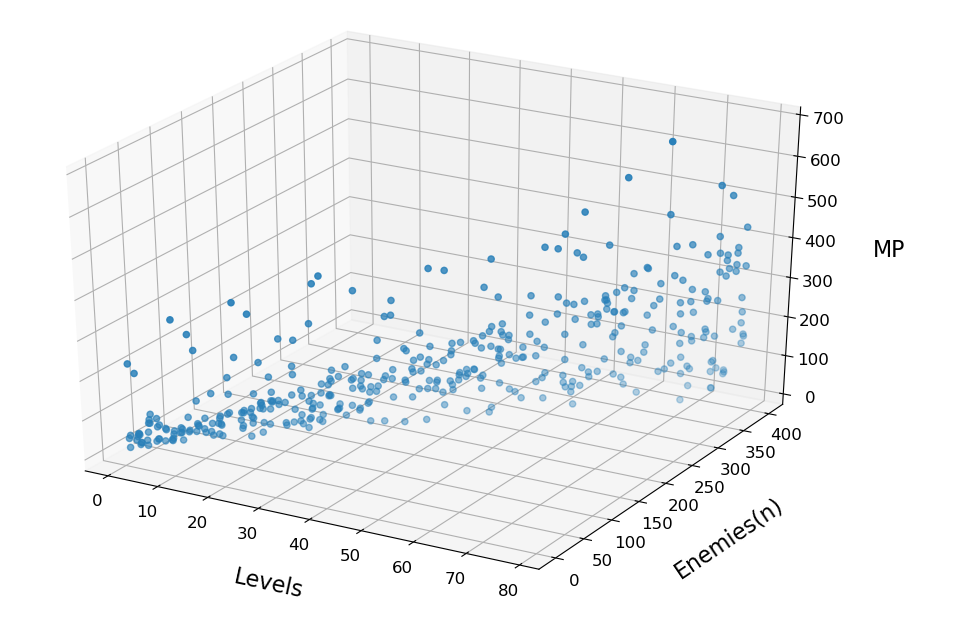
\includegraphics[scale=0.57]{img/EnemyMpDistrib.png}
	\caption{Distribusi \textit{stats} MP musuh.}
	\label{fig:enemy_mp_distrib}
\end{figure}
\vspace{1ex}

Masih pada Sub-bab \ref{sec:sub_sec3_enemy_hp_mp_stats}, dimana pada bagian ini membahas tentang pendistribusian \textit{stats} musuh untuk permaian dengan genre \textit{turn-based} RPG. Berikut adalah hasil dari proses distribusi tipe musuh yang diperoleh dari perhitungan mulai dari persamaan \ref{eq:enemy_types_stats_ex} secara berurutan sampai dengan persamaan \ref{eq:enemy_types_prob_adv} yang digunakan untuk penentuan tipe musuh yang ingin dipakai. Sedangkan proses kalkulasi untuk menentukan \textit{stats} musuh dimulai dari persamaan \ref{eq:enemy_types_prob_bst1} sampai dengan persamaan \ref{eq:enemy_types_prob_st}. Setelah melalui tahapan tersebut dengan variabel masukan pada Tabel \ref{tb:enemy_input_variable} maka hasil persebaran \textit{stats} musuh dengan komposisi \textit{Strength}, \textit{Magic}, \textit{Endurance}, \textit{Speed}, dan \textit{Luck} ditunjukkan pada Tabel \ref{tb:enemy_stats}.
\vspace{-1ex}

\begin{longtable}{|l|l|l|l|l|l|l|l|}
	\caption{Distribusi \textit{Stats} musuh.}
	\label{tb:enemy_stats}\\
	\hline
	\rowcolor[HTML]{C0C0C0} 
	\textbf{No.} & \textbf{Name} & \textbf{Lv.} & \textbf{Str} & \textbf{Mag} & \textbf{Endr} & \textbf{Spd} & \textbf{Luck} \\ \hline
	1 & Enemy 1 & 1 & 2 & 2 & 2 & 2 & 2 \\ \hline
	2 & Enemy 2 & 1 & 2 & 2 & 2 & 2 & 2 \\ \hline
	3 & Enemy 3 & 1 & 2 & 2 & 6 & 2 & 2 \\ \hline
	4 & Enemy 4 & 1 & 2 & 2 & 6 & 2 & 2 \\ \hline
	5 & Enemy 5 & 2 & 2 & 3 & 6 & 3 & 2 \\ \hline
	6 & Enemy 6 & 2 & 2 & 3 & 9 & 2 & 2 \\ \hline
	7 & Enemy 7 & 2 & 2 & 3 & 6 & 2 & 2 \\ \hline
	8 & Enemy 8 & 2 & 2 & 3 & 2 & 2 & 2 \\ \hline
	9 & Enemy 9 & 2 & 2 & 3 & 10 & 3 & 2 \\ \hline
	10 & Enemy 10 & 2 & 2 & 3 & 11 & 3 & 2 \\ \hline
	11 & Enemy 11 & 2 & 2 & 3 & 2 & 2 & 2 \\ \hline
	12 & Enemy 12 & 2 & 2 & 3 & 12 & 3 & 2 \\ \hline
	13 & Enemy 13 & 2 & 2 & 3 & 6 & 2 & 2 \\ \hline
	14 & Enemy 14 & 3 & 2 & 8 & 2 & 2 & 2 \\ \hline
	15 & Enemy 15 & 3 & 3 & 11 & 2 & 3 & 2 \\ \hline
	16 & Enemy 16 & 3 & 2 & 2 & 11 & 2 & 2 \\ \hline
	... & ... & ... & ... & ... & ... & ... & ... \\ \hline
	\textbf{400} & \textbf{Enemy 400} & \textbf{78} & \textbf{30} & \textbf{15} & \textbf{11} & \textbf{36} & \textbf{22} \\ \hline
\end{longtable}
\vspace{1ex}

Selanjutnya adalah penggambaran persebaran \textit{stats} yang disebutkan pada Tabel \ref{tb:enemy_stats} yang digambarkan pada Gambar \ref{fig:enemy_stats_distrib}. Pada Gambar \ref{fig:enemy_str_distrib}, \ref{fig:enemy_mag_distrib}, \ref{fig:enemy_endr_distrib}, \ref{fig:enemy_spd_distrib} dan Gambar \ref{fig:enemy_luck_distrib} adalah pecahan dari Gambar \ref{fig:enemy_stats_distrib} secara berurutan diantaranya adalah \textit{Strength}, \textit{Magic}, \textit{Endurance}, \textit{Speed} dan \textit{Luck}. Data \textit{Stats} selengkapnya dapat dilihat pada \nameref{chap:chap6_attachment} dalam Tabel \ref{tb:enemies_all_stats_1} sampai dengan Tabel \ref{tb:enemies_all_stats_15} pada kolom \textit{Strength}, \textit{Magic}, \textit{Endurance}, \textit{Speed}, \textit{Luck} dan \textit{stats} yang lain jika dilakukan penambahan \textit{stats} pada program. 
\vspace{1ex}

\begin{figure} [!h] \centering
	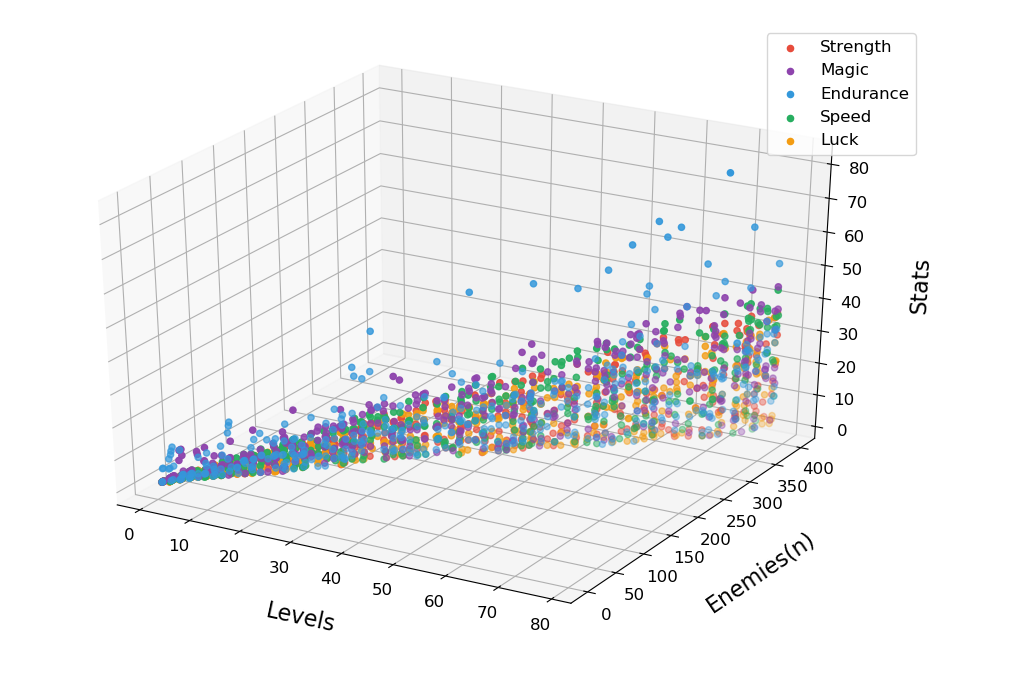
\includegraphics[scale=0.6]{img/EnemyStatsDistrib.png}
	\caption{Distribusi \textit{stats} musuh secara keseluruhan.}
	\label{fig:enemy_stats_distrib}
	\vspace{5ex}
\end{figure}

\begin{figure} [!h] \centering
	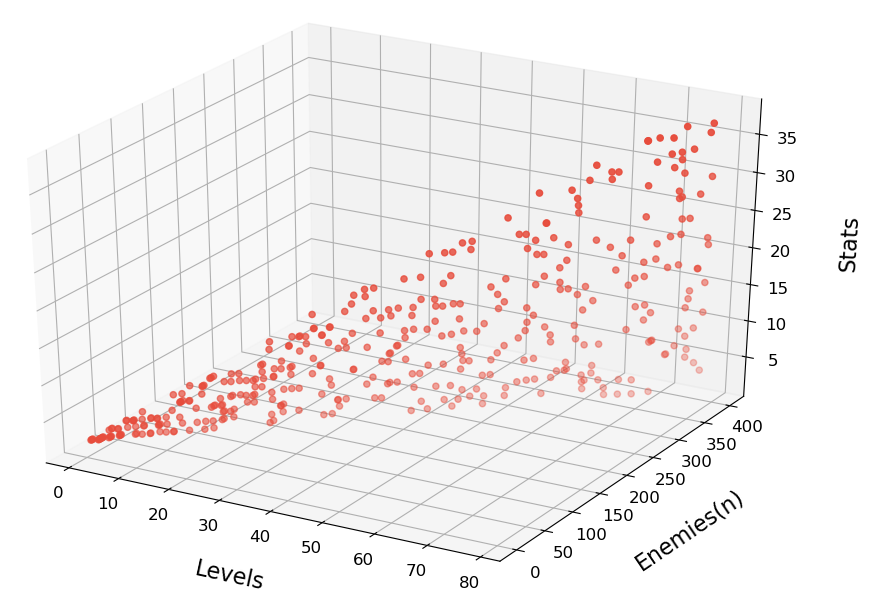
\includegraphics[scale=0.6]{img/EnemyStrengthDistrib.png}
	\caption{Distribusi \textit{Strength} musuh.}
	\label{fig:enemy_str_distrib}
\end{figure}

\begin{figure} [!h] \centering
	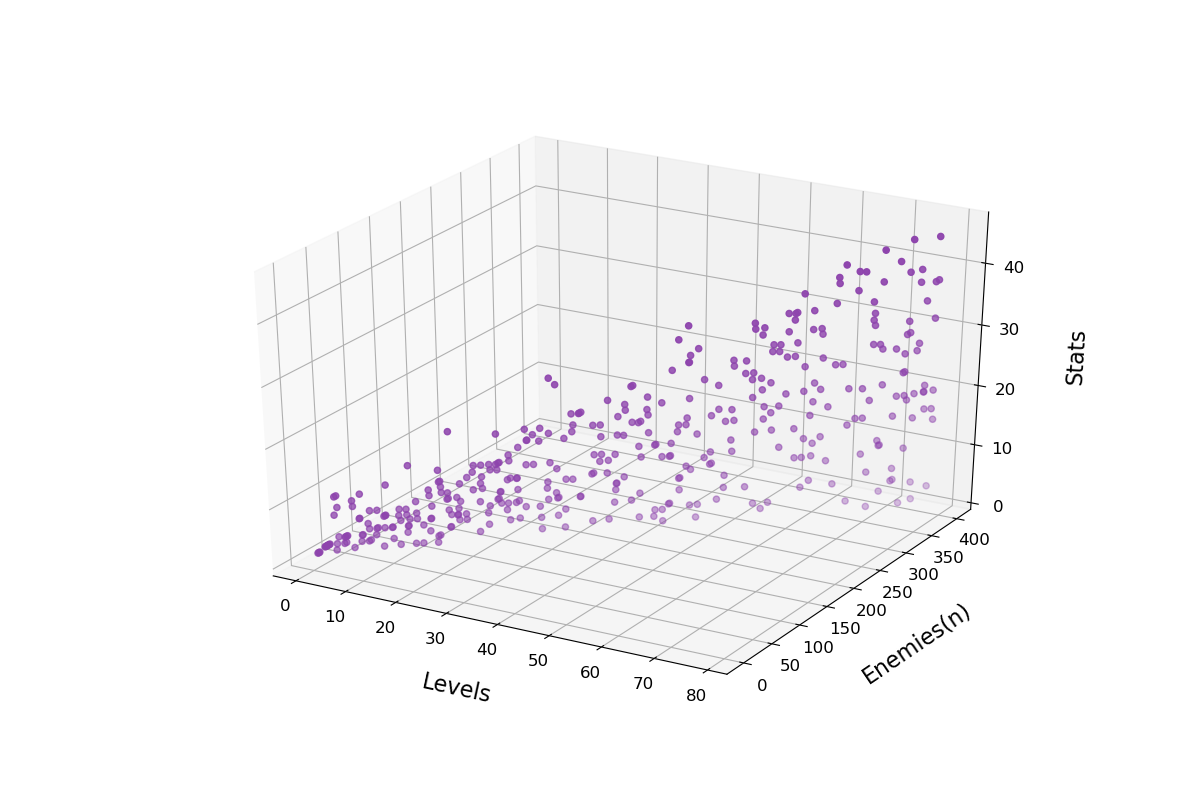
\includegraphics[scale=0.6]{img/EnemyMagicDistrib.png}
	\caption{Distribusi \textit{Magic} musuh.}
	\label{fig:enemy_mag_distrib}
	\vspace{5ex}
\end{figure}

\begin{figure} [!h] \centering
	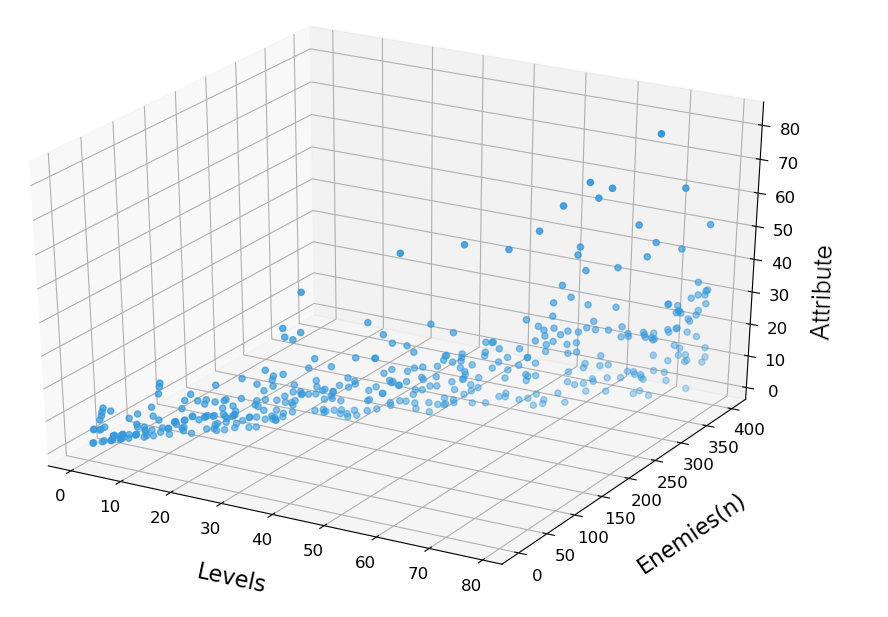
\includegraphics[scale=0.6]{img/EnemyEnduranceDistrib.png}
	\caption{Distribusi \textit{Endurance} musuh.}
	\label{fig:enemy_endr_distrib}
\end{figure}

\begin{figure} [!h] \centering
	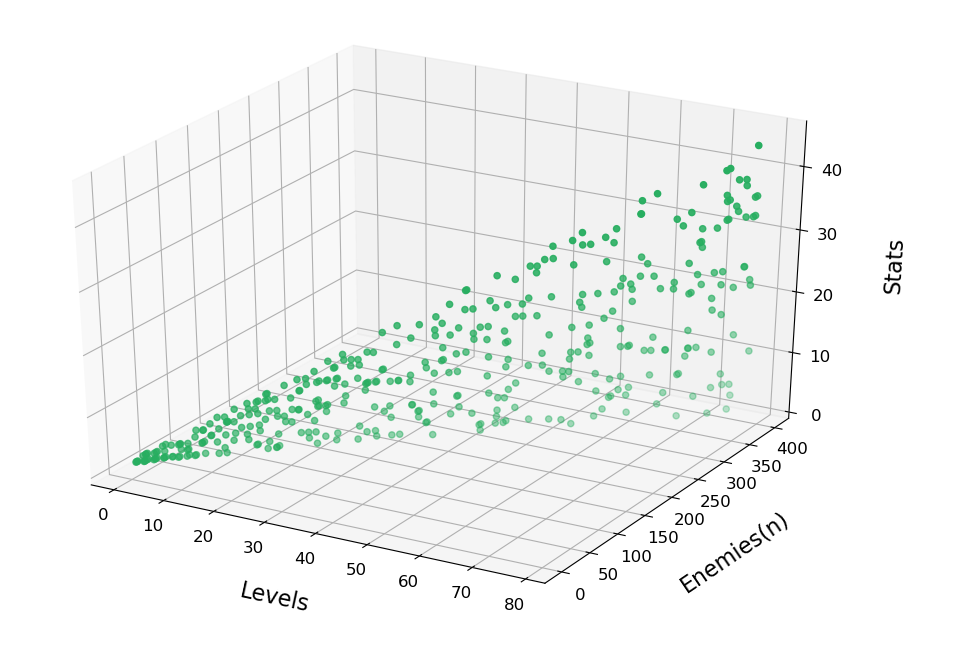
\includegraphics[scale=0.6]{img/EnemySpeedDistrib.png}
	\caption{Distribusi \textit{Speed} musuh.}
	\label{fig:enemy_spd_distrib}
	\vspace{5ex}
\end{figure}

\begin{figure} [!h] \centering
	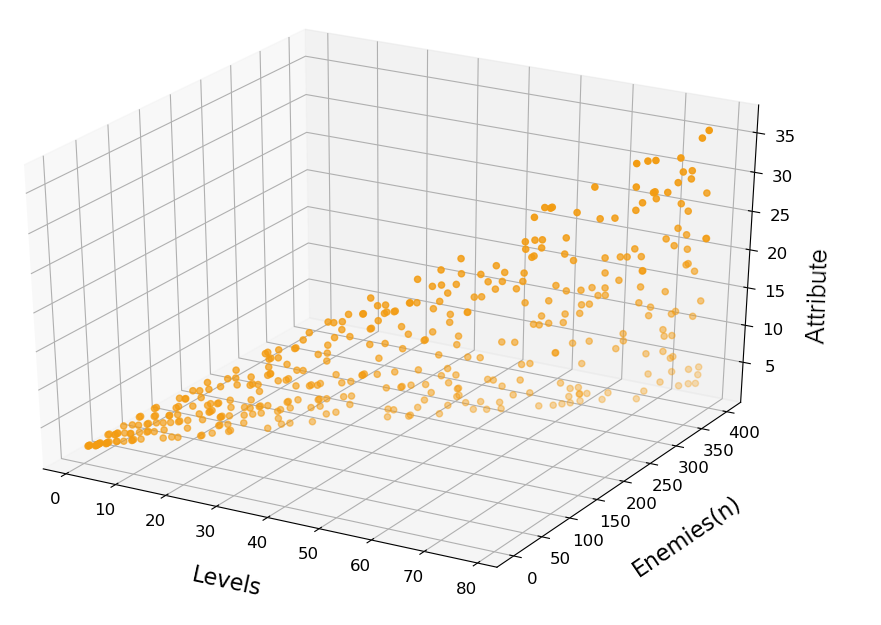
\includegraphics[scale=0.6]{img/EnemyLuckDistrib.png}
	\caption{Distribusi \textit{Luck} musuh.}
	\label{fig:enemy_luck_distrib}
\end{figure}
\vspace{1ex}